\documentclass{vkr}
\usepackage[english, russian]{babel} % переносы
\usepackage{graphicx} % для вставки картинок
\graphicspath{{images/}} % путь к изображениям
\usepackage[hidelinks]{hyperref}
\usepackage{float} % определяет метод H для рисунка с переносом на следующую страницу, ели не помещается
\usepackage{pdflscape}
\addto{\captionsrussian}{\renewcommand{\refname}{СПИСОК ИСПОЛЬЗОВАННЫХ ИСТОЧНИКОВ}}
\usepackage{xltabular} % для вставки таблиц
\usepackage{makecell}
\renewcommand\theadfont{} % шрифт в /thead
\usepackage{array} % для определения новых типов столбцов таблиц
\newcolumntype{T}{>{\centering\arraybackslash}X} % новый тип столбца T - автоматическая ширина столбца с выравниванием по центру
\newcolumntype{R}{>{\raggedleft\arraybackslash}X} % новый тип столбца R - автоматическая ширина столбца с выравниванием по правому краю
\newcolumntype{C}[1]{>{\centering\let\newline\\\arraybackslash\hspace{0pt}}m{#1}} % новый тип столбца C - фиксированная ширина столбца с выравниванием по центру
\newcolumntype{r}[1]{>{\raggedleft\arraybackslash}p{#1}} % новый тип столбца r - фиксированная ширина столбца с выравниванием по правому краю
\newcommand{\centrow}{\centering\arraybackslash} % командой \centrow можно центрировать одну ячейку (заголовок) в столбце типа X или p, оставив в оcтальных ячейках другой тип выравнивания
\newcommand{\finishhead}{\endhead\hline\endlastfoot}
\newcommand{\continuecaption}[1]{\captionsetup{labelformat=empty} \caption[]{#1}\\ \hline }
\usepackage{etoolbox}
\AtBeginEnvironment{xltabular}{\refstepcounter{tablecnt}} % подсчет таблиц xltabular, обычные таблицы подсчитываются в классе

\usepackage[tableposition=top]{caption} % подпись таблицы вверху
\captionsetup{strut=off}
\setlength{\intextsep}{0pt} % Vertical space above & below [h] floats
\setlength{\textfloatsep}{0pt} % Vertical space below (above) [t] ([b]) floats
\DeclareCaptionLabelFormat{gostfigure}{Рисунок #2} %подпись рисунка
\DeclareCaptionLabelFormat{gosttable}{Таблица #2} %подпись таблицы
\DeclareCaptionLabelSeparator{gost}{~--~} %разделитель в рисунках и таблицах
\captionsetup{labelsep=gost}
\captionsetup[figure]{aboveskip=10pt,belowskip=4mm,justification=centering,labelformat=gostfigure} % настройка подписи рисунка
\captionsetup[table]{font={stretch=1.41},skip=0pt,belowskip=0pt,aboveskip=8.5pt,singlelinecheck=off,labelformat=gosttable} % настройка подписи таблицы

\setlength{\LTpre}{8mm} % отступ сверху таблицы
\setlength{\LTpost}{6mm} % отступ снизу таблицы

\usepackage{enumitem}
\setlist{nolistsep,wide=\parindent,itemindent=*} % отступы вокруг списков, выравнивание с учетом разделителя

\usepackage{color} %% это для отображения цвета в коде
\usepackage{listings} %% листинги кода
\setmonofont[Scale=0.7]{Verdana} % моноширный шрифт для листинга

\definecolor{codegreen}{rgb}{0,0.6,0}
\definecolor{codegray}{rgb}{0.5,0.5,0.5}
\definecolor{codepurple}{rgb}{0.58,0,0.82}

\lstset{ %
language=C,                 % выбор языка для подсветки (здесь это С)
numbers=left,               % где поставить нумерацию строк (слева\справа)
numberstyle=\tiny,           % размер шрифта для номеров строк
stepnumber=1,                   % размер шага между двумя номерами строк
numbersep=5pt,                % как далеко отстоят номера строк от подсвечиваемого кода
commentstyle=\color{codegreen},
keywordstyle=\color{magenta},
numberstyle=\tiny\color{codegray},
stringstyle=\color{codepurple},
basicstyle=\linespread{0.95}\ttfamily,
backgroundcolor=\color{white}, % цвет фона подсветки - используем \usepackage{color}
showspaces=false,            % показывать или нет пробелы специальными отступами
showstringspaces=false,      % показывать или нет пробелы в строках
showtabs=false,             % показывать или нет табуляцию в строках
frame=single,              % рисовать рамку вокруг кода
tabsize=2,                 % размер табуляции по умолчанию равен 2 пробелам
captionpos=t,              % позиция заголовка вверху [t] или внизу [b] 
breaklines=true,           % автоматически переносить строки (да\нет)
breakatwhitespace=false, % переносить строки только если есть пробел
escapeinside={\%*}{*)}   % если нужно добавить комментарии в коде
}

\makeatletter % чтобы допускались русские комментарии в листингах
\lst@InputCatcodes
\def\lst@DefEC{%
 \lst@CCECUse \lst@ProcessLetter
  ^^80^^81^^82^^83^^84^^85^^86^^87^^88^^89^^8a^^8b^^8c^^8d^^8e^^8f%
  ^^90^^91^^92^^93^^94^^95^^96^^97^^98^^99^^9a^^9b^^9c^^9d^^9e^^9f%
  ^^a0^^a1^^a2^^a3^^a4^^a5^^a6^^a7^^a8^^a9^^aa^^ab^^ac^^ad^^ae^^af%
  ^^b0^^b1^^b2^^b3^^b4^^b5^^b6^^b7^^b8^^b9^^ba^^bb^^bc^^bd^^be^^bf%
  ^^c0^^c1^^c2^^c3^^c4^^c5^^c6^^c7^^c8^^c9^^ca^^cb^^cc^^cd^^ce^^cf%
  ^^d0^^d1^^d2^^d3^^d4^^d5^^d6^^d7^^d8^^d9^^da^^db^^dc^^dd^^de^^df%
  ^^e0^^e1^^e2^^e3^^e4^^e5^^e6^^e7^^e8^^e9^^ea^^eb^^ec^^ed^^ee^^ef%
  ^^f0^^f1^^f2^^f3^^f4^^f5^^f6^^f7^^f8^^f9^^fa^^fb^^fc^^fd^^fe^^ff%
  ^^^^20ac^^^^0153^^^^0152%
  % Basic Cyrillic alphabet coverage
  ^^^^0410^^^^0411^^^^0412^^^^0413^^^^0414^^^^0415^^^^0416^^^^0417%
  ^^^^0418^^^^0419^^^^041a^^^^041b^^^^041c^^^^041d^^^^041e^^^^041f%
  ^^^^0420^^^^0421^^^^0422^^^^0423^^^^0424^^^^0425^^^^0426^^^^0427%
  ^^^^0428^^^^0429^^^^042a^^^^042b^^^^042c^^^^042d^^^^042e^^^^042f%
  ^^^^0430^^^^0431^^^^0432^^^^0433^^^^0434^^^^0435^^^^0436^^^^0437%
  ^^^^0438^^^^0439^^^^043a^^^^043b^^^^043c^^^^043d^^^^043e^^^^043f%
  ^^^^0440^^^^0441^^^^0442^^^^0443^^^^0444^^^^0445^^^^0446^^^^0447%
  ^^^^0448^^^^0449^^^^044a^^^^044b^^^^044c^^^^044d^^^^044e^^^^044f%
  ^^^^0401^^^^0451%
  %%%
  ^^00}
\lst@RestoreCatcodes
\makeatother

% Режим шаблона (должен быть включен один из трех)
% \ВКРtrue
\Практикаtrue
%\Курсоваяtrue

\newcommand{\Дисциплина}{<<Проектирование и архитектура программных систем>>} % для курсовой
\newcommand{\КодСпециальности}{09.03.04} % Курсовая
\newcommand{\Специальность}{Программная инженерия} % Курсовая
\newcommand{\Тема}{Разработка web-сайта «Русатом – Аддитивные технологии» на платформе} % ВКР Курсовая
\newcommand{\ТемаВтораяСтрока}{1С-Битрикс}
\newcommand{\ГдеПроводитсяПрактика}{ОАО <<Какао-Какао>>} % для практики
\newcommand{\РуководительПрактПредпр}{Иванов И. И.} % для практики
\newcommand{\ДолжнРуководительПрактПредпр}{директор} % для практики
\newcommand{\РуководительПрактУнивер}{Иванов И. И.} % для практики
\newcommand{\ДолжнРуководительПрактУнивер}{к.т.н. доцент} % для практики
\newcommand{\Автор}{И. И. Иванов}
\newcommand{\АвторРод}{Иванов И.И.}
\newcommand{\АвторПолностьюРод}{Иванова И.И.} % для практики
\newcommand{\Шифр}{XX-XX-XXXX}
\newcommand{\Курс}{4} % для практики
\newcommand{\Группа}{XX-XXX}
\newcommand{\Руководитель}{И. И. Иванов} % для ВКР и курсовой
\newcommand{\Нормоконтроль}{И. И. Иванов} % для ВКР
\newcommand{\ЗавКаф}{И. И. Иванов} % для ВКР
\newcommand{\ДатаПриказа}{«07» апреля 2023~г.} % для ВКР
\newcommand{\НомерПриказа}{1505-с} % для ВКР
\newcommand{\СрокПредоставления}{«13» июня 2023~г.} % для ВКР, курсового

% \usepackage{xcolor}
\begin{document}
% \pagecolor{black!90}
% \color{black!10}
\maketitle
\ifПрактика{}\else{
   \newpage
\begin{center}
\large\textbf{Минобрнауки России}

\large\textbf{Юго-Западный государственный университет}
\vskip 1em
\normalsize{Кафедра программной инженерии}
\vskip 1em
\ifВКР{
        \begin{flushright}
        \begin{tabular}{p{.4\textwidth}}
        \centrow УТВЕРЖДАЮ: \\
        \centrow Заведующий кафедрой \\
        \hrulefill \\
        \setarstrut{\footnotesize}
        \centrow\footnotesize{(подпись, инициалы, фамилия)}\\
        \restorearstrut
        «\underline{\hspace{1cm}}»
        \underline{\hspace{3cm}}
        20\underline{\hspace{1cm}} г.\\
        \end{tabular}
        \end{flushright}
        }\fi
\end{center}
\vspace{1em}
  \begin{center}
  \large
\ifВКР{
ЗАДАНИЕ НА ВЫПУСКНУЮ КВАЛИФИКАЦИОННУЮ РАБОТУ
  ПО ПРОГРАММЕ БАКАЛАВРИАТА}
  \else
ЗАДАНИЕ НА КУРСОВУЮ РАБОТУ (ПРОЕКТ)
\fi
\normalsize
  \end{center}
\vspace{1em}
{\parindent0pt
  Студента \АвторРод, шифр\ \Шифр, группа \Группа
  
1. Тема «\Тема\ \ТемаВтораяСтрока»
\ifВКР{
утверждена приказом ректора ЮЗГУ от \ДатаПриказа\ № \НомерПриказа
}\fi.

2. Срок предоставления работы к защите \СрокПредоставления

3. Исходные данные для создания программной системы:

3.1. Перечень решаемых задач:}

\renewcommand\labelenumi{\theenumi)}

\begin{enumerate}
\item проанализировать современные технологии и подходы к разработке графических движков;
\item разработать архитектуру кроссплатформенного графического движка для визуализации трёхмерных сцен;
\item реализовать основные компоненты графического конвейера с использованием OpenGL и SDL2;
\item разработать систему управления шейдерами, текстурами и геометрическими примитивами;
\item реализовать систему камеры и освещения сцены;
\item разработать формат файлов сцены и систему их загрузки;
\item провести тестирование и оптимизацию работы движка.
\end{enumerate}

{\parindent0pt
  3.2. Входные данные и требуемые результаты для программы:}

\begin{enumerate}
\item Входными данными для программной системы являются: структура сцены с описанием объектов, источников света и камеры, текстуры в формате пиксельных данных, вершинные и фрагментные шейдеры на специализированном языке GLSL, ввод из пользовательского приложения.
\item Выходными данными для программной системы являются: трёхмерная сцена, визуализируемая в реальном времени, обработанные пользовательские события управления сценой, журналы работы приложения и отладочная информация.
\end{enumerate}

{\parindent0pt

  4. Содержание работы (по разделам):

  4.1. Введение.

  4.2. Анализ предметной области.

  4.3. Техническое задание: основание для разработки, цель и назначение разработки, требования к программной системе, требования к оформлению документации.

  4.4. Технический проект: общая характеристика архитектуры решения, проектирование архитектурных компонентов программной системы, проектирование основных сущностей программной системы.

  4.5. Рабочий проект: спецификация компонентов и классов программной системы, тестирование программной системы, сборка компонентов программной системы.  % TODO:

  4.6. Заключение.

  4.7. Список использованных источников.

5. Перечень графического материала:

\списокПлакатов

\vskip 2em
\begin{tabular}{p{6.8cm}C{3.8cm}C{4.8cm}}
Руководитель \ifВКР{ВКР}\else работы (проекта) \fi & \lhrulefill{\fill} & \fillcenter\Руководитель\\
\setarstrut{\footnotesize}
& \footnotesize{(подпись, дата)} & \footnotesize{(инициалы, фамилия)}\\
\restorearstrut
Задание принял к исполнению & \lhrulefill{\fill} & \fillcenter\Автор\\
\setarstrut{\footnotesize}
& \footnotesize{(подпись, дата)} & \footnotesize{(инициалы, фамилия)}\\
\restorearstrut
\end{tabular}
}

\renewcommand\labelenumi{\theenumi.}

   \abstract{РЕФЕРАТ}

Объем работы равен \formbytotal{lastpage}{страниц}{е}{ам}{ам}. Работа содержит \formbytotal{figurecnt}{иллюстраци}{ю}{и}{й}, \formbytotal{tablecnt}{таблиц}{у}{ы}{}, \arabic{bibcount} библиографических источников и \formbytotal{числоПлакатов}{лист}{}{а}{ов} графического материала. Количество приложений – 2. Графический материал представлен в приложении А. Фрагменты исходного кода представлены в приложении Б.

Перечень ключевых слов: графический движок, рендеринг, OpenGL, компьютерная графика, трёхмерная визуализация, шейдеры, текстуры, геометрия, камера, освещение, кроссплатформенность, SDL2, GLSL, GLM, C++, графический конвейер, прямая отрисовка, отложенная отрисовка, матрицы преобразований, буферы вершин, буферы индексов.

Объектом разработки является информационная система для визуализации трёхмерных сцен, реализованная на языке C++ с использованием современных графических технологий.

Целью выпускной квалификационной работы является разработка кроссплатформенного графического движка, обеспечивающего эффективный рендеринг трёхмерных сцен в реальном времени с использованием современных технологий компьютерной графики.

В процессе разработки были реализованы следующие основные компоненты: подсистема управления окнами и вводом, графический конвейер на базе OpenGL 3.3, система загрузки и управления шейдерами, подсистема работы с геометрией и текстурами, система камеры и освещения сцены, менеджер сцен и объектов.

Движок демонстрирует высокую производительность при рендеринге сложных трёхмерных сцен и может быть использован в различных областях, включая разработку интерактивных приложений, научную визуализацию и образовательные проекты.

\selectlanguage{english}
\abstract{ABSTRACT}
  
The volume of work is \formbytotal{lastpage}{page}{}{s}{s}. The work contains \formbytotal{figurecnt}{illustration}{}{s}{s}, \formbytotal{tablecnt}{table}{}{s}{s}, \arabic{bibcount} bibliographic sources and \formbytotal{числоПлакатов}{sheet}{}{s}{s} of graphic material. The number of applications is 2. The graphic material is presented in annex A. The layout of the site, including the connection of components, is presented in annex B.

List of keywords: graphics engine, rendering, OpenGL, computer graphics, 3D visualization, shaders, textures, geometry, camera, lighting, cross-platform, SDL2, GLSL, GLM, C++, graphics pipeline, deferred rendering, forward rendering, transformation matrices, vertex buffers, index buffers.

The object of development is a graphics engine for 3D scene visualization, implemented in C++ using modern graphics technologies.

The purpose of the final qualifying work is to develop a cross-platform graphics engine that provides efficient real-time rendering of 3D scenes using modern computer graphics technologies.

During the development, the following main components were implemented: window and input management subsystem, graphics pipeline based on OpenGL 3.3, shader loading and management system, geometry and texture handling subsystem, scene camera and lighting system, scene and object manager.

The engine demonstrates high performance in rendering complex 3D scenes and can be used in various fields, including interactive application development, scientific visualization, and educational projects.
\selectlanguage{russian}
}\fi
\tableofcontents
\section*{ОБОЗНАЧЕНИЯ И СОКРАЩЕНИЯ}

Графический движок -- приложение или компонент приложения, отвечающий за обработку виртуальных графических объектов и вывод их изображения на экран.

Рендеринг -- процесс обработки двух- или трёхмерного объекта и вывода его проекции на экран.

Спрайты -- двухмерные графические объекты.

Ray casting -- <<бросание лучей>>, простейший метод определения видимости объектов в 3D-сцене.

Ray tracing -- трассировка лучей, метод определения видимости объектов в 3D-сцене, основанный на физических закономерностях светового распространения.

API (Application Programming Interface) -- интерфейс программирования приложений.

Кроссплатформенность -- возможность использования одного и того же приложения на разных платформах (операционных системах).

Скриптинг -- задание логики и поведения объектов в сцене.

Сцена -- абстрактное представление совокупности объектов, взаимодействующих между собой и обрабатываемых движком одновременно.

VBO (Vertex Buffer Object) -- объект буфера вершин.

VAO (Vertex Array Object) -- объект массива вершин.

EBO (Element Buffer Object) -- объект буфера элементов.

ИС -- информационная система.

ИТ -- информационные технологии.

КТС -- комплекс технических средств.

ПО -- программное обеспечение.

ОС -- операционная система.

РП -- рабочий проект.

ТЗ -- техническое задание.

ТП -- технический проект.

UML (Unified Modelling Language) -- язык графического описания для объектного моделирования в области разработки программного обеспечения.

\ifПрактика{}\else{\section*{ВВЕДЕНИЕ}
\addcontentsline{toc}{section}{ВВЕДЕНИЕ}

Современные технологии визуализации трёхмерной графики нашли широкое применение в различных областях: от компьютерных игр и кинематографа до научной визуализации и проектирования. Одним из ключевых компонентов, обеспечивающих работу с 3D-графикой, являются графические движки — специализированные программные комплексы, отвечающие за рендеринг трёхмерных сцен в реальном времени.

Графический движок представляет собой сложную систему, включающую в себя подсистемы для работы с геометрией, материалами, текстурами, освещением, анимацией и другими аспектами компьютерной графики. Современные движки должны обеспечивать высокую производительность, кроссплатформенность и гибкость при работе с различными типами контента.

В последние годы наблюдается растущий спрос на специализированные решения для визуализации, которые могут быть интегрированы в существующие информационные системы предприятий. Это требует от разработчиков создания модульных, расширяемых и хорошо документированных решений, способных работать в различных окружениях.

Разрабатываемый в рамках данной работы графический движок ставит своей целью предоставить простое в использовании, но мощное решение для визуализации трёхмерных сцен. Движок построен на базе современных технологий, обеспечивающих кроссплатформенность и высокую производительность.

\emph{Целью настоящей работы} является разработка кроссплатформенного графического движка для визуализации трёхмерных сцен с использованием современных технологий рендеринга. Для достижения поставленной цели необходимо решить \emph{следующие задачи}:
\begin{itemize}
\item проанализировать современные технологии и подходы к разработке графических движков;
\item разработать архитектуру кроссплатформенного графического движка;
\item реализовать основные компоненты графического конвейера;
\item разработать систему управления шейдерами, текстурами и геометрическими примитивами;
\item реализовать систему камеры и освещения сцены;
\item разработать формат файлов сцены и систему их загрузки;
\item провести тестирование и оптимизацию работы движка.
\end{itemize}

\emph{Структура и объем работы.} Отчет состоит из введения, 4 разделов основной части, заключения, списка использованных источников, 2 приложений. Текст выпускной квалификационной работы равен \formbytotal{lastpage}{страниц}{е}{ам}{ам}.

\emph{Во введении} сформулирована цель работы, поставлены задачи разработки, описана структура работы, приведено краткое содержание каждого из разделов.

\emph{В первом разделе} на стадии описания технической характеристики предметной области приводится анализ современных технологий и подходов к разработке графических движков.

\emph{Во втором разделе} на стадии технического задания приводятся требования к разрабатываемому движку.

\emph{В третьем разделе} на стадии технического проектирования представлены проектные решения для движка.

\emph{В четвертом разделе} приводится список классов и их методов, использованных при разработке движка, производится тестирование разработанного движка.

В заключении излагаются основные результаты работы, полученные в ходе разработки.

В приложении А представлен графический материал.
В приложении Б представлены фрагменты исходного кода. 
}\fi
\section{Анализ предметной области}
\subsection{Характеристика предприятия и его деятельности}

Компания ООО <<Предприятие ВТИ-Сервис>> является ведущим интегратором корпоративных информационных систем, специализируясь на внедрении и сопровождении решений на платформе 1С, а также системном администрировании сложных ИТ-инфраструктур. Основанная в 1996 году, компания активно развивает направление автоматизации бизнес-процессов и создания специализированного программного обеспечения для своих клиентов.

В современном мире компьютерная графика играет важнейшую роль в различных областях: от игровой индустрии до научных исследований. Технологии рендеринга трёхмерных объектов прошли долгий путь развития от простых каркасных моделей до фотореалистичных изображений с динамическим освещением. Важнейшим этапом в этой эволюции стало появление графических API, таких как OpenGL и DirectX, которые позволили разработчикам создавать высокопроизводительные приложения для визуализации 3D-графики.

Термин <<графический движок>> (англ. rendering engine) обозначает программный комплекс, предназначенный для визуализации виртуальных сцен. Современные графические движки предоставляют широкий спектр возможностей: от базовой отрисовки геометрических примитивов до сложных систем освещения, текстурирования и физического моделирования. Они являются фундаментальным инструментом в разработке интерактивных приложений и игр.

Графические движки находят применение во множестве областей: разработка компьютерных игр, архитектурная визуализация, кинематограф, научная визуализация данных, системы виртуальной и дополненной реальности, тренажеры и симуляторы. Каждая из этих областей предъявляет свои требования к функциональности и производительности движков.

В рамках преддипломной практики под руководством ООО <<Предприятие ВТИ-Сервис>> был создан графический движок REngine, предназначенный для интеграции с корпоративными системами визуализации данных. Движок использует технологии OpenGL и SDL2, обеспечивающие кроссплатформенность и возможность встраивания в существующие ИТ-инфраструктуры клиентов. Данное решение может быть использовано для создания специализированных интерфейсов визуализации производственных процессов, интеграции с системами бизнес-аналитики и другими корпоративными решениями.

\subsection{История развития графических движков}

Эволюция графических движков тесно связана с развитием аппаратного обеспечения и графических API. Можно выделить несколько ключевых этапов:

\begin{enumerate}
    \item 1980-1989 гг. -- появление первых примитивных движков для аркадных автоматов и домашних компьютеров. Графика была исключительно двумерной, использовались спрайты и плиточные карты.
    \item 1990-1999 гг. -- с появлением первых 3D-ускорителей начинается эра трёхмерной графики. Знаковые движки этого периода:
    \begin{itemize}[itemindent=\parindent,leftmargin=\parindent]
        \item Wolfenstein 3D engine (1992) -- первый движок с псевдо-3D графикой, использующий технологию ray casting;
        \item Doom engine (1993) -- развитие предыдущего движка, дополняющее его вертикальной видимостью;
        \item Quake engine (1996) -- первый полностью трёхмерный движок с аппаратным ускорением;
        \item Unreal Engine (1998) -- ввел концепции визуального редактора сцен и скриптинга.
    \end{itemize}
    \item 2000-2009 гг. -- стандартизация графических API (OpenGL, DirectX), появление шейдеров и программируемого конвейера, развитие middleware -- программ-посредников (OGRE, Irrlicht).
    \item 2010-2019 гг. -- доминирование коммерческих движков (Unity, Unreal Engine 4), развитие мобильной графики (OpenGL ES), появление новых API (Vulkan, Metal).
    \item 2020-н.в. -- акцент на фотореализм с использованием аппаратно ускоренной трассировки лучей (ray tracing), виртуальную реальность (VR) и кроссплатформенность, растет спрос на специализированные движки для бизнес-приложений и визуализации данных.
\end{enumerate}

В корпоративном секторе графические движки находят применение в:
\begin{itemize}
    \item системах визуализации производственных процессов;
    \item инструментах бизнес-аналитики и BI-системах;
    \item тренажерах и симуляторах для промышленности;
    \item системах проектирования и прототипирования.
\end{itemize}

\subsection{Графические движки и технологии рендеринга}

Основное преимущество использования графических движков заключается в абстрагировании от низкоуровневых деталей работы с графическим API. Разработчик получает готовый инструментарий для создания и визуализации трёхмерных сцен, что существенно сокращает время разработки и позволяет сосредоточиться на логике приложения.

Современные графические движки можно классифицировать по нескольким критериям.

По используемому графическому API:
\begin{itemize}
    \item OpenGL -- обеспечивает совместимость с наиболее широким количеством платформ;
    \item DirectX -- оптимизирован для работы на машинах под управлением Microsoft Windows;
    \item Vulkan -- является наследником OpenGL и обеспечивает низкоуровневый доступ к графическому оборудованию для наибольшей производительности;
    \item Metal -- разработан специально для устройств Apple.
\end{itemize}

По типу рендеринга:
\begin{itemize}
    \item движки с отложенным рендерингом (Deferred Rendering) -- позволяют эффективно обрабатывать сложные графические сцены с большим количеством источников света;
    \item движки с прямым рендерингом (Forward Rendering) -- обеспечивают высокую производительность при упрощённых графических сценах;
    \item гибридные решения, сочетающие преимущества обоих подходов.
\end{itemize}

По специализации:
\begin{itemize}
    \item универсальные движки -- подходят для широкого спектра задач;
    \item специализированные движки -- оптимизированы для конкретных типов приложений (игры, научная визуализация и т.д.);
    \item движки реального времени -- обеспечивают мгновенную визуализацию изменений в сцене.
\end{itemize}

Движок REngine относится к категории универсальных OpenGL-движков с прямым рендерингом, что обеспечивает оптимальный баланс между производительностью и качеством визуализации для широкого спектра приложений.

\section{Техническое задание}
\subsection{Основание для разработки}

Полное наименование системы: <<Программная система для визуализации объектов в трёхмерном пространстве>>.

Основанием для разработки является приказ ректора ЮЗГУ от <<17>> апреля 2025 г. №1828-с <<О направлении (допуске) на практику>>.

\subsection{Цель и назначение разработки}

Основной целью преддипломной практики является разработка программной системы (графического движка) для визуализации трёхмерных данных в реальном времени для ООО <<Предприятие ВТИ-Сервис>>.

Посредством разработки данного движка планируется решить ряд технических задач, стоящих перед компанией. Цели разработки можно разделить на две основные группы: технические и практические.

Задачами данной разработки являются:

\begin{enumerate}
    \item Реализация базовых компонентов графического конвейера на основе OpenGL.
    \item Создание кроссплатформенного решения с использованием SDL2.
    \item Разработка системы управления шейдерами и текстурами.
    \item Реализация системы камеры.
    \item Создание базовых геометрических примитивов.
    \item Разработка формата файлов сцены.
    \item Разработка системы загрузки и отображения сцен.
\end{enumerate}

\subsection{Требования к программной системе}

\subsubsection{Требования к интерфейсу пользователя}

Интерфейс пользователя должен быть максимально простым для концентрации на визуализации трёхмерных объектов. Один из вариантов внешнего вида окна программы представлен на рисунке \ref{interface:image}.

\begin{figure}[ht]
\center{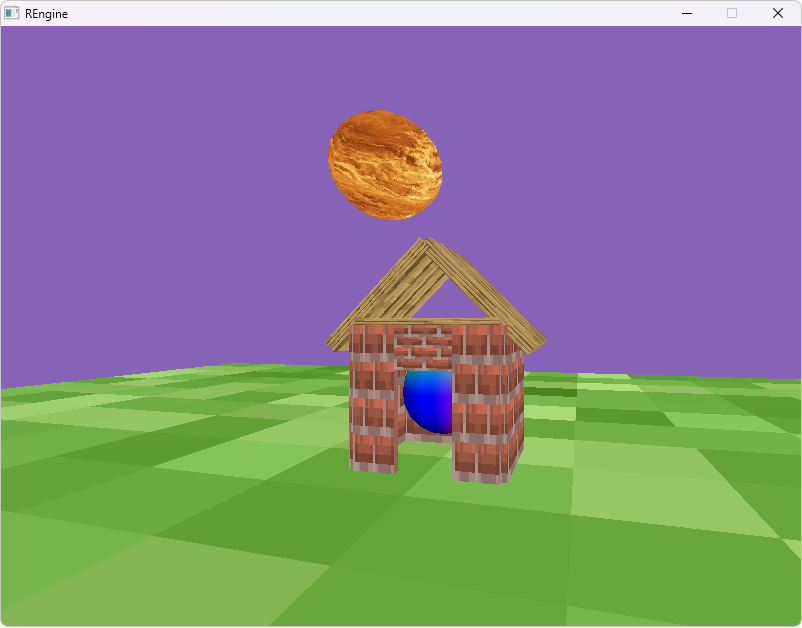
\includegraphics[width=1\linewidth]{screenshot.png}}
\caption{Окно программы}
\label{interface:image}
\end{figure}

\subsubsection{Функциональные требования}

Для разрабатываемого графического движка была построена модель, отражающая основные сценарии его использования в корпоративной среде.

Данная модель помогает выявить ключевые точки интеграции движка с существующими информационными системами предприятия, а также определить роли пользователей и взаимодействие с внешними системами. Для описания сценариев используется унифицированный язык визуального моделирования UML.

Диаграмма вариантов использования описывает функциональное назначение разрабатываемой системы. Она является исходным концептуальным представлением системы в процессе ее проектирования и разработки. Проектируемая система представляется в виде ряда прецедентов, предоставляемых системой актерам или сущностям, которые взаимодействуют с системой. Актером или действующим лицом является сущность, взаимодействующая с системой извне (например, человек, техническое устройство). Прецедент служит для описания набора действий, которые система предоставляет актеру.

На основании анализа предметной области в программе должны быть реализованы следующие прецеденты:

\begin{enumerate}
    \item Отображение заранее созданных трёхмерных сцен с базовыми геометрическими примитивами (кубы, сферы).
    \item Перемещение камеры по трёхмерной сцене с помощью клавиатуры и мыши.
    \item Загрузка и применение текстур к объектам.
    \item Изменение вершинных и фрагментных шейдеров.
    \item Кроссплатформенная работа на операционных системах Windows и Linux.
\end{enumerate}

На рисунке \ref{usecase:image} представлена диаграмма вариантов использования.

\begin{figure}[ht]
\center{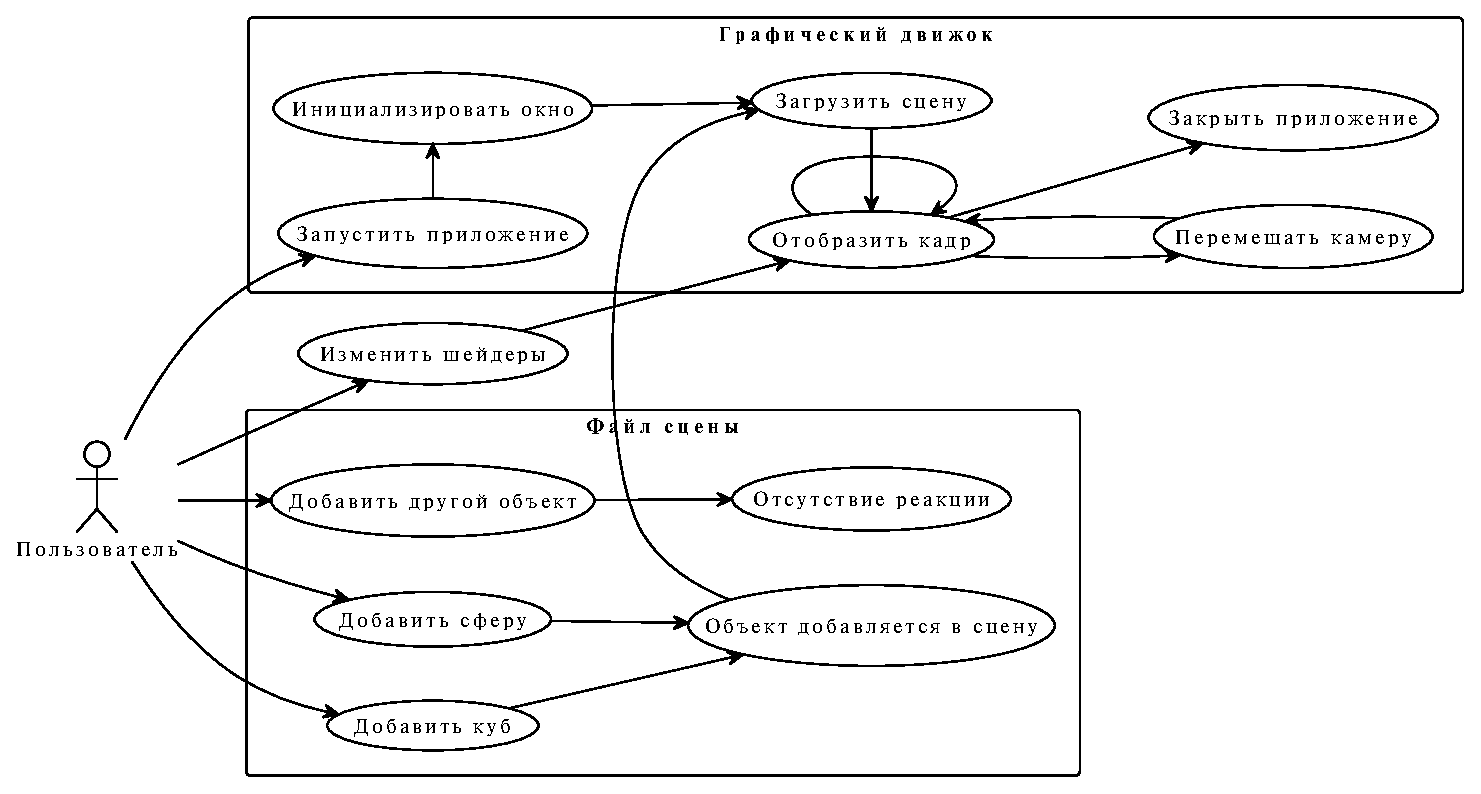
\includegraphics[width=1\linewidth]{usecase}}
\caption{Диаграмма вариантов использования}
\label{usecase:image}
\end{figure}

\paragraph{Вариант использования <<Отображение трёхмерной сцены>>}

Заинтересованные лица и их требования: пользователь желает увидеть трёхмерную сцену. Предусловие: запущена поддерживаемая операционная система, файл сцены присутствует, шейдеры стандартные. Постусловие: пользователь ознакомляется с визуализацией.

\begin{enumerate}
    \item Пользователь запускает приложение.
    \item Приложение инициализирует графический контекст.
    \item Приложение компилирует шейдеры.
    \item Приложение загружает файл сцены.
    \item Приложение создаёт геометрические примитивы.
    \item Приложение отображает трёхмерную сцену.
    \item Пользователь видит трёхмерную сцену.
\end{enumerate}

\paragraph{Вариант использования <<Перемещение камеры>>}

Заинтересованные лица и их требования: пользователь желает перемещать камеру по трёхмерной сцене. Предусловие: запущена поддерживаемая операционная система, файл сцены присутствует, шейдеры стандартные. Постусловие: пользователь имеет возможность увидеть трёхмерную сцену под другим ракурсом.

\begin{enumerate}
    \item Пользователь запускает приложение.
    \item Приложение инициализирует графический контекст.
    \item Приложение компилирует шейдеры.
    \item Приложение загружает файл сцены.
    \item Приложение создаёт геометрические примитивы.
    \item Приложение отображает трёхмерную сцену.
    \item Пользователь нажимает на клавиши клавиатуры и двигает мышью для перемещения камеры в пространстве.
    \item Приложение обрабатывает ввод и изменяет матрицу вида камеры.
    \item Пользователь видит изменение перспективы камеры.
\end{enumerate}

\paragraph{Вариант использования <<Изменение сцены>>}

Заинтересованные лица и их требования: пользователь желает добавить несколько объектов в трёхмерную сцену. Предусловие: запущена поддерживаемая операционная система, файл сцены присутствует, шейдеры стандартные, текстуры существуют. Постусловие: пользователь видит изменённую его руками трёхмерную сцену.

\begin{enumerate}
    \item Пользователь открывает файл сцены.
    \item Пользователь добавляет объект типа <<куб>> в сцену.
    \item Пользователь добавляет объект типа <<сфера>> в сцену.
    \item Пользователь добавляет объект типа <<цилиндр>> в сцену.
    \item Пользователь изменяет начальное положение камеры.
    \item Пользователь добавляет путь к текстуре к созданному объекту <<куб>>.
    \item Пользователь запускает приложение.
    \item Приложение инициализирует графический контекст.
    \item Приложение компилирует шейдеры.
    \item Приложение загружает файл сцены.
    \item Приложение игнорирует объект типа <<цилиндр>>, поскольку он не реализован в программе.
    \item Приложение загружает текстуру по указанному пути и применяет её к объекту <<куб>>.
    \item Приложение создаёт геометрические примитивы.
    \item Приложение отображает трёхмерную сцену.
    \item Пользователь видит трёхмерную сцену.
\end{enumerate}

\paragraph{Вариант использования <<Изменение шейдеров>>}

Заинтересованные лица и их требования: пользователь желает изменить шейдеры, применяемые для отображения объектов в трёхмерной сцене. Предусловие: запущена поддерживаемая операционная система, файл сцены присутствует, шейдеры стандартные. Постусловие: пользователь видит трёхмерную сцену с изменёнными шейдерами.

\begin{enumerate}
    \item Пользователь изменяет вершинный шейдер в соответствии с спецификацией языка GLSL.
    \item Пользователь изменяет фрагментный шейдер в соответствии с спецификацией языка GLSL.
    \item Пользователь запускает приложение.
    \item Приложение инициализирует графический контекст.
    \item Приложение компилирует шейдеры.
    \item Приложение загружает файл сцены.
    \item Приложение создаёт геометрические примитивы.
    \item Приложение отображает трёхмерную сцену.
    \item Пользователь видит трёхмерную сцену с визуальными изменениями, соответствующими изменённым шейдерам.
\end{enumerate}

\subsection{Нефункциональные требования к программной системе}

\subsubsection{Требования к программному обеспечению}

Для реализации разрабатываемого движка должны использоваться языки программирования C++ и GLSL, компилятор GCC и система сборки CMake.

Для запуска и работы с движком требуется использование компьютера под управлением 64-битной операционной системы Windows 7 (или выше) или Linux.

\subsubsection{Требования к аппаратному обеспечению}

Клиентское оборудование должно иметь центральный процессор с частотой ядра не менее 1 ГГц и поддержкой SSE2, а также видеокарту с поддержкой OpenGL 3.3 или выше. Объём оперативной памяти -- 512 ГБ.

Доступ к сети Интернет не требуется.

\subsection{Требования к оформлению документации}

Разработка программной документации и программного изделия должна производиться согласно ГОСТ 19.102-77 и ГОСТ 34.601-90. Единая система программной документации.

\section{Технический проект}
\subsection{Общая характеристика архитектуры решения}

Графический движок представляет собой кроссплатформенное приложение для визуализации трёхмерных сцен, построенное на следующих ключевых компонентах:

\begin{itemize}
    \item подсистема управления окнами (SDL2);
    \item графический конвейер (OpenGL 3.3);
    \item подсистема загрузки ресурсов (текстуры, шейдеры);
    \item менеджер сцен и объектов.
\end{itemize}

Движок спроектирован как модульная система, позволяющая расширять функционал без изменения ядра.

\subsection{Обоснование выбора технологий}

\subsubsection{Язык программирования C++}

В качестве основного языка разработки выбран C++ -- высокопроизводительный компилируемый язык, обеспечивающий прямой доступ к API библиотек. Его кроссплатформенная природа позволяет компилировать движок под различные операционные системы без изменения исходного кода. Современные стандарты C++ предоставляют необходимые средства для эффективной работы с памятью и многопоточностью, что критично для графических приложений.

\subsubsection{Система сборки CMake}

В качестве системы управления сборкой в проекте применяется CMake, что обусловлено его гибкостью и широкой поддержкой в индустрии разработки программного обеспечения. Использование CMake позволяет централизованно описывать структуру проекта, автоматически находить и подключать сторонние библиотеки, а также формировать корректные проекты для различных платформ и сред разработки. Современные стандарты CMake делают сборочный процесс прозрачным и легко масштабируемым: добавление новых исходных файлов или зависимостей не требует ручных изменений для каждой платформы.

Использование подобной системы минимизирует вероятность ошибок, связанных с различиями между платформами, и ускоряет процесс разработки.

\subsubsection{Компилятор GCC}

Для компиляции движка был выбран бесплатный компилятор с открытым исходным кодом GCC (GNU Compiler Collection), обеспечивающий возможность компиляции C и C++ кода с поддержкой современных стандартов. GCC по-умолчанию поддерживается только на операционной системе Linux, но имеет возможность компиляции под Windows с помощью MinGW.

\subsubsection{Набор инструментов разработки MinGW}

Для сборки и запуска проекта на платформе Windows используется набор инструментов разработки MinGW (Minimalist GNU for Windows), который предоставляет среду для работы с GCC. Он также обеспечивает совместимость с другими инструментами Linux, что облегчает переносимость кода между платформами, а также позволяют использовать единые скрипты сборки и тестирования.

В процессе разработки данного проекта MinGW показал себя как надёжное и удобное решение для удобной разработки под Windows.

\subsubsection{Библиотека SDL2}

Для взаимодействия с оконной системой используется библиотека SDL2 (Simple DirectMedia Layer), которая абстрагирует платформозависимые особенности создания окон, обработки ввода и работы с аудио. SDL2 была выбрана благодаря своей стабильности, поддержке нескольких платформ и минимальным затратам времени на адаптацию. Библиотека предоставляет простой API для инициализации графического контекста OpenGL и обработки пользовательского ввода.

\subsubsection{Спецификация графического API OpenGL}

Графический конвейер реализован на основе OpenGL 3.3 Core Profile -- кроссплатформенного графического API, поддерживаемого большинством современных видеокарт. Выбор версии 3.3 обусловлен балансом между функциональностью и совместимостью: этот стандарт предоставляет современный конвейер рендеринга с шейдерной моделью, но при этом не требует новейшей аппаратуры.

Для привязки аппаратных функций OpenGL к структурам языка C++ используется загрузочная библиотека Glad.

OpenGL был предпочтен Vulkan и Direct3D ввиду своей универсальности и меньшего порога входа.

\subsubsection{Язык программирования шейдеров GLSL}

GLSL (OpenGL Shading Language) является языком программирования для написания шейдеров, используемых в конвейере рендеринга. Шейдеры позволяют конечным пользователям настраивать различные аспекты визуализации, такие как текстуры, освещение и эффекты, без перекомпиляции основной части программы. Все операции шейдеров выполняются на графическом ускорителе, что обеспечивает высокую производительность.

\subsubsection{Математическая библиотека GLM}

Библиотека GLM (OpenGL Mathematics) предоставляет математические функции и типы данных, специфичные для компьютерной графики:

\begin{itemize}
    \item операции с векторами и матрицами (произведение, сложение, вычитание);
    \item трансформации (перемещение, вращение, масштабирование);
    \item пространственных преобразований (нормализация, проекции).
\end{itemize}

GLM применяется в движке для упрощения таких действий, как расчёт матриц модели, вида и проекции, преобразование координат и управление камерой и перспективой.

Библиотека была выбрана благодаря полной совместимости с OpenGL, оптимизированным SIMD-операциям и удобному синтаксису, аналогичному GLSL.

\subsection{Архитектурные компоненты системы}

Диаграмма компонентов (рис. \ref{comp:image}) отражает физическую и логическую структуру графического движка. Архитектура системы построена по принципу разделения ответственности, где каждый компонент инкапсулирует строго определённую функциональность.

\afterpage{
  \begin{landscape}
    \begin{figure}[p]
      \centering
      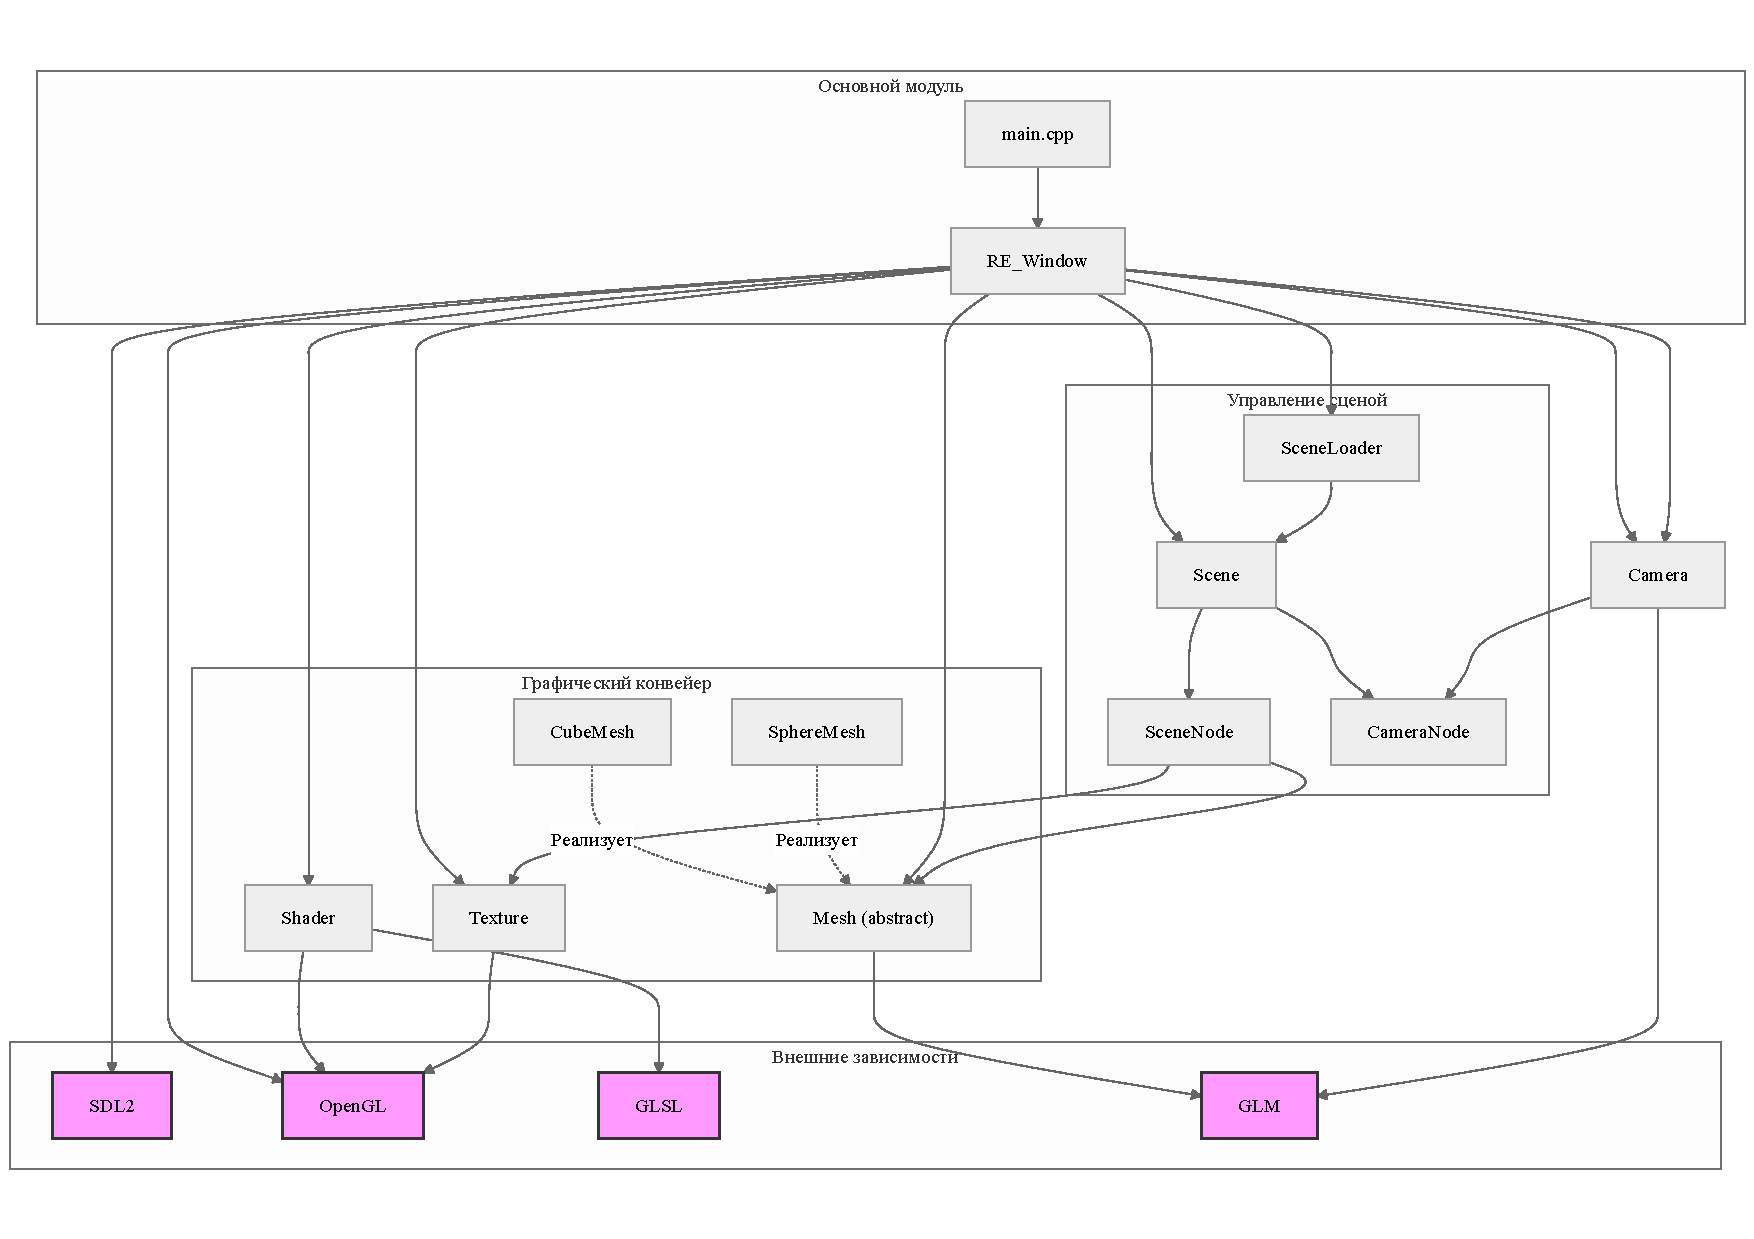
\includegraphics[width=1.6\textwidth]{comp.pdf}
      \caption{Диаграмма компонентов движка с последовательностью взаимодействия}
      \label{comp:image}
    \end{figure}
  \end{landscape}
}

\subsubsection{Состав компонентов}

Основные модули системы включают:

\begin{enumerate}
    \item Window -- компонент управления окном, реализующий:

    \begin{itemize}[itemindent=\parindent,leftmargin=\parindent]
        \item инициализацию окна;
        \item обработку ввода;
        \item обработку событий.
    \end{itemize}

    \item Renderer -- компонент управления конвейером рендеринга, реализующий абстракцию над API OpenGL. Обеспечивает:

    \begin{itemize}[itemindent=\parindent,leftmargin=\parindent]
        \item инициализацию контекста OpenGL;
        \item загрузку шейдеров;
        \item управление сценой;
        \item отрисовку сцены.
    \end{itemize}

    \item Scene -- подсистема работы со сценой:

    \begin{itemize}[itemindent=\parindent,leftmargin=\parindent]
        \item хранит коллекцию объектов (SceneNode) и управляет их состоянием;
        \item хранит камеру и параметры освещения;
        \item поддерживает цвет неба (skyColor), параметры направленного и точечных источников света (DirLight, PointLight), а также масштабируемое количество источников света.
    \end{itemize}

    \item InputHandler -- компонент обработки пользовательского ввода:

    \begin{itemize}[itemindent=\parindent,leftmargin=\parindent]
        \item предоставляет интерфейс для регистрации callback-функций на нажатие, удержание и отпускание клавиш;
        \item поддерживает обработку событий мыши (движение, нажатие, прокрутка);
        \item хранит состояния клавиш и мыши;
        \item обеспечивает получение текущей позиции и относительного перемещения мыши.
    \end{itemize}

    \item Графический конвейер (неявный компонент):

    \begin{itemize}[itemindent=\parindent,leftmargin=\parindent]
        \item Shader -- управление шейдерными программами (вершинный/фрагментный);
        \item Texture -- загрузка, генерация и привязка текстурных объектов;
        \item Mesh -- хранение геометрических данных (VBO/VAO/EBO).
    \end{itemize}

    \item Camera -- компонент управления видами, реализующий:

    \begin{itemize}[itemindent=\parindent,leftmargin=\parindent]
        \item расчёт матриц вида и проекции;
        \item преобразование координат;
        \item управление параметрами отображения (позиция, углы, FOV);
        \item относительное перемещение и вращение;
        \item получение и установка углов поворота.
    \end{itemize}
\end{enumerate}

\subsubsection{Взаимодействие компонентов}

Последовательность работы системы (рис. \ref{comp:image}) реализуется следующим образом:

\begin{enumerate}
    \item Инициализация:

    \begin{itemize}[itemindent=\parindent,leftmargin=\parindent]
        \item Renderer создаёт графический контекст;
        \item Shader компилирует шейдерные программы;
        \item Клиентская программа создаёт начальную сцену, используя компонент Scene.
    \end{itemize}

    \item Главный цикл рендеринга:

    \begin{itemize}[itemindent=\parindent,leftmargin=\parindent]
        \item обновление матриц вида в Camera;
        \item передача uniform-переменных в шейдеры;
        \item формирование вершинного буфера объектов сцены из вектора SceneNode;
        \item отрисовка объектов сцены с учётом их:

        \begin{itemize}[itemindent=\parindent,leftmargin=\parindent]
            \item геометрии (Mesh);
            \item текстуры (Texture);
            \item шейдеров (Shader).
        \end{itemize}

        \item вывод результата через Renderer;
        \item обработка пользовательского ввода Renderer и передача его значений в Camera;
        \item повтор цикла до выхода из программы.
    \end{itemize}
\end{enumerate}

\ifПрактика{}\else{
   \section{Рабочий проект}

\subsection{Классы, используемые при разработке сайта}

Программная система состоит из сущностей, выраженных классами и структурами языка C++. Их взаимодействие реализуется через встроенные механизмы наследования и представлено в диаграмме UML (рис. \ref{uml:image}).

\afterpage{
  \begin{landscape}
    \begin{figure}[p]
      \centering
      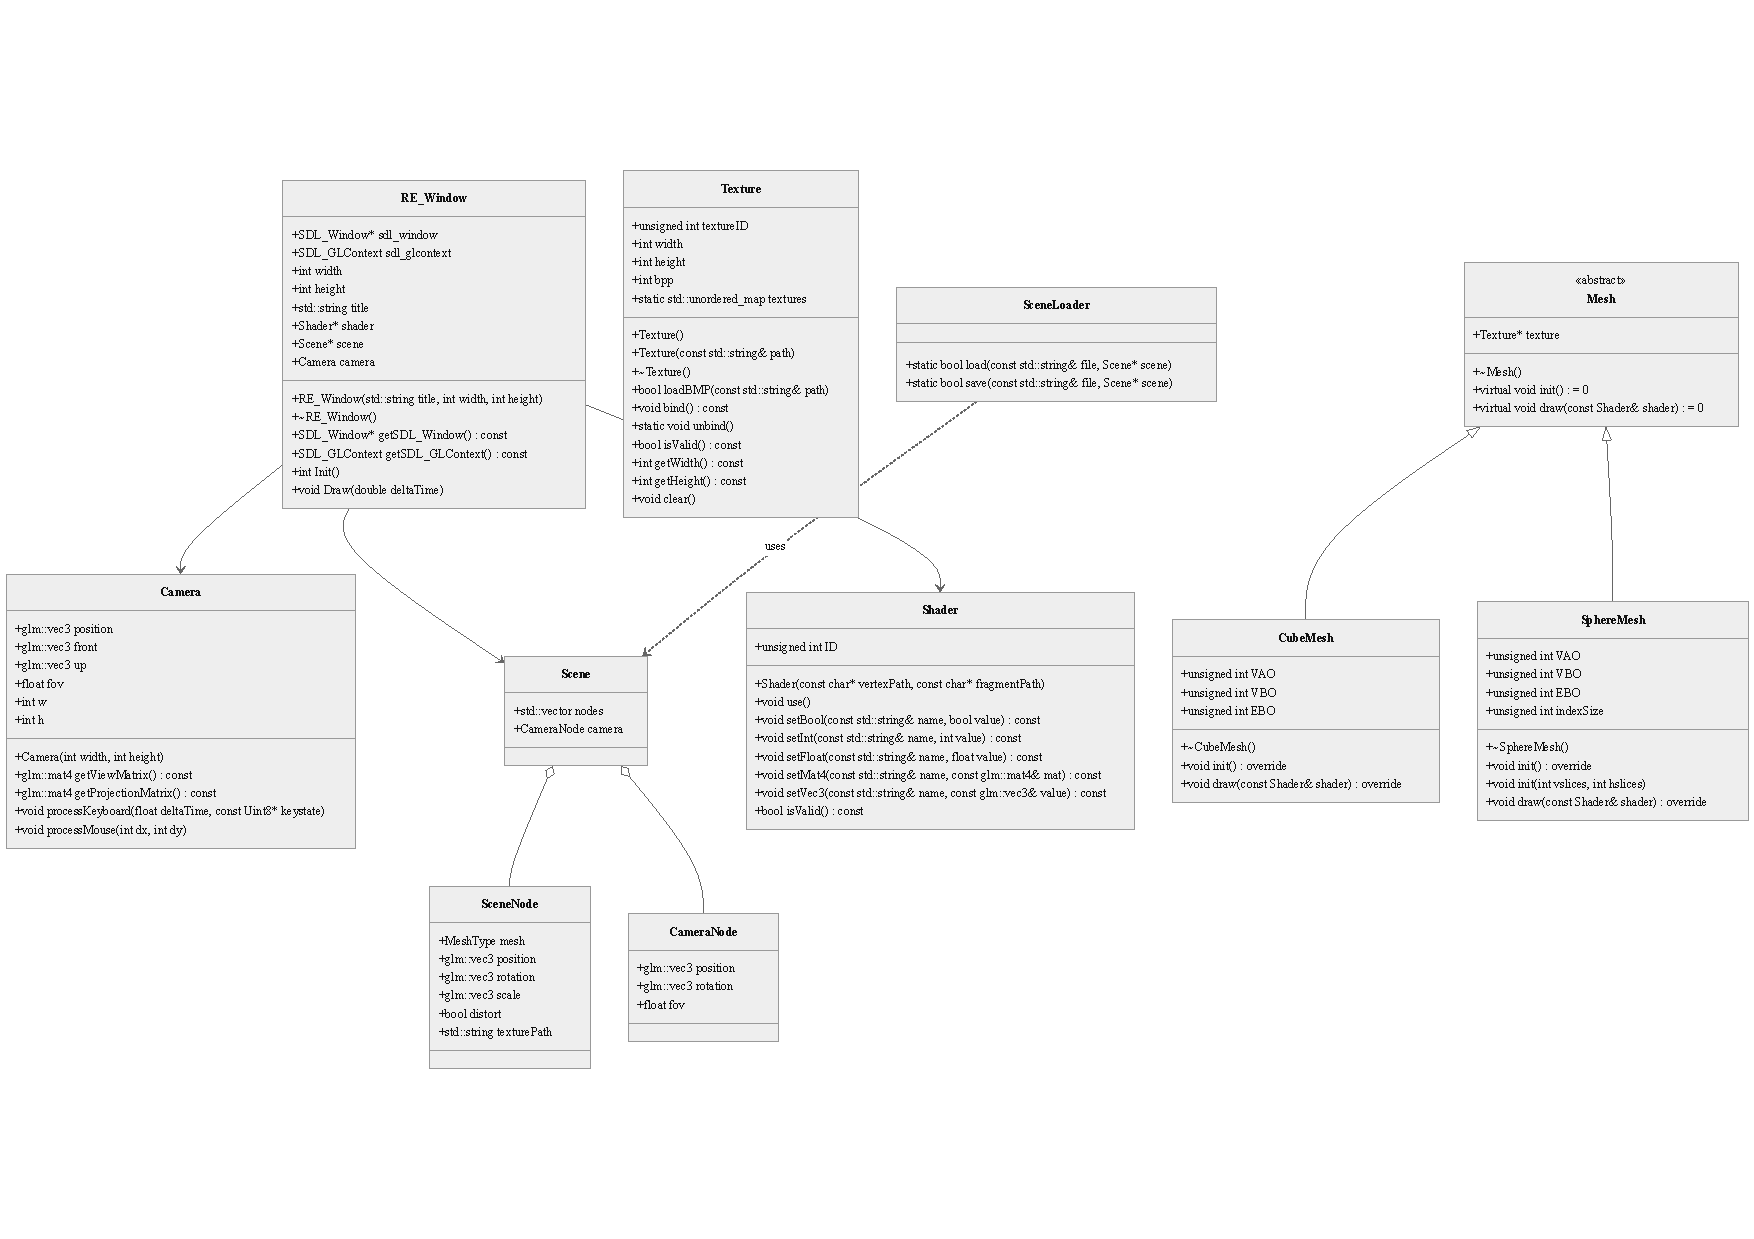
\includegraphics[width=1.6\textwidth]{uml.pdf}
      \caption{Диаграмма UML}
      \label{uml:image}
    \end{figure}
  \end{landscape}
}

\subsubsection{Класс Renderer}
Класс Renderer отвечает за управление процессом отрисовки трёхмерной сцены. Он инкапсулирует логику взаимодействия с графическим API (OpenGL), управляет объектами сцены, шейдерами и камерой. Класс не занимается напрямую созданием окна или обработкой событий, предполагая, что эти задачи решаются внешними компонентами.

Спецификация класса Renderer представлена в таблице \ref{tab:renderer_spec}.

\begin{xltabular}{\textwidth}{|X|l|X|}
    \caption{Спецификация класса Renderer\label{tab:renderer_spec}}\\ \hline
    \centrow Поле/Метод & \centrow Тип & \centrow Описание \\ \hline
    \endfirsthead
    \continuecaption{Продолжение таблицы \ref{tab:renderer_spec}}
    \centrow Поле/Метод & \centrow Тип & \centrow Описание \\ \hline 
    \finishhead

    \multicolumn{3}{|l|}{Приватные поля} \\ \hline
    width & int & Ширина области рендеринга в пикселях. \\ \hline
    height & int & Высота области рендеринга в пикселях. \\ \hline
    scene & Scene* & Указатель на объект сцены, содержащий все объекты для отображения. \\ \hline
    \multicolumn{3}{|l|}{Методы} \\ \hline
    Renderer(int width, int height) & конструктор & Конструктор класса. Инициализирует размеры области рендеринга. \\ \hline
    getScene() & Scene* & Возвращает указатель на текущую сцену. \\ \hline
    setScene(Scene* scene) & void & Устанавливает активную сцену для рендеринга. \\ \hline
    setShader(const char* vertexPath, const char* fragmentPath) & void & Загружает и устанавливает шейдерную программу по путям к вершинному и фрагментному шейдерам. \\ \hline
    getWidth() & int & Возвращает ширину области рендеринга. \\ \hline
    getHeight() & int & Возвращает высоту области рендеринга. \\ \hline
    draw(unsigned long ticks) & void & Выполняет отрисовку одного кадра. ticks -- текущее время в миллисекундах. \\ \hline
\end{xltabular}

Вспомогательная функция \texttt{initRenderer(int width, int height)} (определена в пространстве имен REngine, заголовочный файл \texttt{Renderer.h}) создает и возвращает указатель на новый экземпляр класса \texttt{Renderer}, инициализированный с заданной шириной и высотой.

\subsubsection{Управление окном и главный цикл}
Функциональность, связанная с созданием окна приложения, управлением главным циклом и закрытием окна, сосредоточена в пространстве имен \texttt{REngine} (см. заголовочный файл \texttt{Engine.h}). Этот модуль предоставляет набор функций и перечисление для кодов ошибок.

\paragraph{Перечисление WindowError}
Перечисление \texttt{WindowError} определяет константы для кодов ошибок, которые могут возникнуть при операциях с окном.

Спецификация перечисления WindowError представлена в таблице \ref{tab:windowerror_spec}.

\begin{xltabular}{\textwidth}{|l|X|}
    \caption{Спецификация перечисления WindowError\label{tab:windowerror_spec}}\\ \hline
    \centrow Значение & \centrow Описание \\ \hline
    \endfirsthead
    \continuecaption{Продолжение таблицы \ref{tab:windowerror_spec}}
    \centrow Значение & \centrow Описание \\ \hline 
    \finishhead
    WINDOW\_ALREADY\_EXISTS & Окно уже было создано. \\ \hline
    WINDOW\_CREATE\_FAILED & Не удалось создать окно SDL. \\ \hline
    GL\_CONTEXT\_CREATE\_FAILED & Не удалось создать контекст OpenGL. \\ \hline
    RENDERER\_INIT\_FAILED & Не удалось инициализировать рендерер. \\ \hline
\end{xltabular}

\paragraph{Функции управления окном}
Набор функций для управления жизненным циклом окна и приложения.

Спецификация функций управления окном представлена в таблице \ref{tab:windowfuncs_spec}.

\begin{xltabular}{\textwidth}{|X|l|X|}
    \caption{Спецификация функций управления окном\label{tab:windowfuncs_spec}}\\ \hline
    \centrow Функция & \centrow Возвращаемый тип & \centrow Описание \\ \hline
    \endfirsthead
    \continuecaption{Продолжение таблицы \ref{tab:windowfuncs_spec}}
    \centrow Функция & \centrow Возвращаемый тип & \centrow Описание \\ \hline 
    \finishhead
    createWindow(const char* title, int width = 0, int height = 0) & int & Инициализирует SDL, создает окно приложения и контекст OpenGL. \texttt{title} - заголовок окна. \texttt{width} и \texttt{height} - размеры окна; если 0, используется полноэкранный режим. Возвращает 0 при успехе или код ошибки из \texttt{WindowError} при неудаче. \\ \hline
    mainLoop() & void & Запускает главный цикл приложения. В цикле обрабатываются события ввода, обновляется состояние сцены и происходит отрисовка. Цикл продолжается до тех пор, пока не будет получен сигнал о закрытии окна. \\ \hline
    setScene(REngine::Scene* scene) & void & Устанавливает текущую сцену для рендеринга. \\ \hline
    getScene() & REngine::Scene* & Возвращает указатель на текущую сцену. \\ \hline
    setShader(const char* vertexPath, const char* fragmentPath) & void & Устанавливает шейдерную программу для рендеринга. \\ \hline
    destroyWindow() & void & Удаляет окно SDL, контекст OpenGL и освобождает ресурсы SDL. Должна вызываться перед завершением работы приложения. \\ \hline
\end{xltabular}

\subsubsection{Структура SceneNode}
Структура \texttt{SceneNode} представляет собой отдельный объект (узел) в трехмерной сцене. Она содержит информацию о геометрии объекта, его трансформациях (позиция, поворот, масштаб), материале и текстурах.

Спецификация структуры SceneNode представлена в таблице \ref{tab:scenenode_spec}.

\begin{xltabular}{\textwidth}{|l|l|X|}
    \caption{Спецификация структуры SceneNode\label{tab:scenenode_spec}}\\ \hline
    \centrow Поле & \centrow Тип & \centrow Описание \\ \hline
    \endfirsthead
    \continuecaption{Продолжение таблицы \ref{tab:scenenode_spec}}
    \centrow Поле & \centrow Тип & \centrow Описание \\ \hline 
    \finishhead
    mesh & Mesh* & Указатель на объект геометрии (меш). \\ \hline
    position & glm::vec3 & Позиция объекта в мировых координатах. Значение по умолчанию: (0,0,0). \\ \hline
    rotation & glm::vec3 & Углы поворота объекта вокруг осей X, Y, Z в градусах. Значение по умолчанию: (0,0,0). \\ \hline
    scale & glm::vec3 & Масштаб объекта по осям X, Y, Z. Значение по умолчанию: (1,1,1). \\ \hline
    shininess & float & Коэффициент блеска материала объекта. Используется в модели освещения Фонга. Значение по умолчанию: 32.0. \\ \hline
    distort & bool & Флаг, указывающий, нужно ли применять эффект искажения к текстуре объекта. Значение по умолчанию: false. \\ \hline
    texturePath & std::string & Путь к файлу основной текстуры объекта (diffuse map). \\ \hline
    specularPath & std::string & Путь к файлу текстуры для карты отражений (specular map). \\ \hline
\end{xltabular}

\subsubsection{Структура DirLight}
Структура \texttt{DirLight} описывает параметры направленного источника света в сцене.

Спецификация структуры DirLight представлена в таблице \ref{tab:dirlight_spec}.

\begin{xltabular}{\textwidth}{|l|l|X|}
    \caption{Спецификация структуры DirLight\label{tab:dirlight_spec}}\\ \hline
    \centrow Поле & \centrow Тип & \centrow Описание \\ \hline
    \endfirsthead
    \continuecaption{Продолжение таблицы \ref{tab:dirlight_spec}}
    \centrow Поле & \centrow Тип & \centrow Описание \\ \hline 
    \finishhead
    direction & glm::vec3 & Вектор направления света. \\ \hline
    ambient & glm::vec3 & Интенсивность окружающего света. Компоненты (R,G,B) в диапазоне [0,1]. \\ \hline
    diffuse & glm::vec3 & Интенсивность диффузного света. Компоненты (R,G,B) в диапазоне [0,1]. \\ \hline
    specular & glm::vec3 & Интенсивность зеркального света. Компоненты (R,G,B) в диапазоне [0,1]. \\ \hline
\end{xltabular}

\subsubsection{Структура PointLight}
Структура \texttt{PointLight} описывает параметры точечного источника света. Точечный свет излучается из одной точки во всех направлениях, и его интенсивность убывает с расстоянием.

Спецификация структуры PointLight представлена в таблице \ref{tab:pointlight_spec}.

\begin{xltabular}{\textwidth}{|l|l|X|}
    \caption{Спецификация структуры PointLight\label{tab:pointlight_spec}}\\ \hline
    \centrow Поле & \centrow Тип & \centrow Описание \\ \hline
    \endfirsthead
    \continuecaption{Продолжение таблицы \ref{tab:pointlight_spec}}
    \centrow Поле & \centrow Тип & \centrow Описание \\ \hline 
    \finishhead
    position & glm::vec3 & Позиция источника света в мировых координатах. \\ \hline
    constant & float & Константный коэффициент затухания интенсивности света. \\ \hline
    linear & float & Линейный коэффициент затухания интенсивности света. \\ \hline
    quadratic & float & Квадратичный коэффициент затухания интенсивности света. \\ \hline
    ambient & glm::vec3 & Цвет окружающего света. \\ \hline
    diffuse & glm::vec3 & Цвет диффузного света. \\ \hline
    specular & glm::vec3 & Цвет зеркального света. \\ \hline
\end{xltabular}

\subsubsection{Класс Camera}
Класс Camera отвечает за управление виртуальной камерой в трехмерном пространстве. Он предоставляет методы для установки и получения позиции и ориентации камеры, вычисления матриц вида и проекции, а также для относительного перемещения и вращения. Камера использует библиотеку GLM для математических операций.

Спецификация класса Camera представлена в таблице \ref{tab:camera_spec}.

\begin{xltabular}{\textwidth}{|X|l|X|}
    \caption{Спецификация класса Camera\label{tab:camera_spec}}\\ \hline
    \centrow Поле/Метод & \centrow Тип & \centrow Описание \\ \hline
    \endfirsthead
    \continuecaption{Продолжение таблицы \ref{tab:camera_spec}}
    \centrow Поле/Метод & \centrow Тип & \centrow Описание \\ \hline 
    \finishhead

    \multicolumn{3}{|l|}{Поля} \\ \hline
    position & glm::vec3 & Позиция камеры в мировых координатах. \\ \hline
    fov & float & Угол обзора (поле зрения) камеры в градусах. \\ \hline
    w & int & Ширина окна отрисовки, используется для расчета матрицы проекции. \\ \hline
    h & int & Высота окна отрисовки, используется для расчета матрицы проекции. \\ \hline
    front & glm::vec3 & (Приватное) Вектор, указывающий направление камеры. \\ \hline
    up & glm::vec3 & (Приватное) Вектор, указывающий "верх" для камеры. \\ \hline
    \multicolumn{3}{|l|}{Методы} \\ \hline
    Camera() & конструктор & Конструктор по умолчанию. \\ \hline
    Camera(int width, int height) & конструктор & Конструктор. Инициализирует камеру с указанной шириной и высотой окна. \\ \hline
    setRotation(float rx, float ry, float rz) & void & Устанавливает углы поворота камеры по осям X, Y, Z (в градусах). \\ \hline
    getRotation() const & glm::vec3 & Возвращает текущие углы поворота камеры по осям X, Y, Z (в градусах) в виде вектора. \\ \hline
    getViewMatrix() const & glm::mat4 & Вычисляет и возвращает матрицу вида (view matrix). \\ \hline
    getProjectionMatrix() const & glm::mat4 & Вычисляет и возвращает матрицу проекции (projection matrix). \\ \hline
    moveRelative(float dx, float dy, float dz) & void & Перемещает камеру относительно ее текущей ориентации на заданные смещения. \\ \hline
    rotateRelative(float drx, float dry, float drz) & void & Поворачивает камеру относительно ее текущей ориентации на заданные углы (в градусах). \\ \hline
\end{xltabular}

\subsubsection{Структура Scene}
Структура \texttt{Scene} является контейнером для всех элементов, составляющих трехмерную сцену. Она объединяет информацию об объектах, камере, источниках света и других параметрах окружения.

Спецификация структуры Scene представлена в таблице \ref{tab:scene_spec}.

\begin{xltabular}{\textwidth}{|l|l|X|}
    \caption{Спецификация структуры Scene\label{tab:scene_spec}}\\ \hline
    \centrow Поле & \centrow Тип & \centrow Описание \\ \hline
    \endfirsthead
    \continuecaption{Продолжение таблицы \ref{tab:scene_spec}}
    \centrow Поле & \centrow Тип & \centrow Описание \\ \hline 
    \finishhead
    nodes & std::vector<SceneNode> & Список всех объектов (узлов) в сцене. \\ \hline
    camera & Camera & Конфигурация камеры сцены. \\ \hline
    skyColor & glm::vec3 & Цвет неба (фона) сцены. Компоненты (R,G,B) в диапазоне [0,1]. Значение по умолчанию: (0.63, 0.63, 0.85). \\ \hline
    dirLight & DirLight & Параметры направленного источника света в сцене. \\ \hline
    pointLights & std::vector<PointLight> & Список точечных источников света в сцене. \\ \hline
\end{xltabular}

\subsubsection{Перечисление MeshType}
Перечисление \texttt{MeshType} определяет типы геометрических примитивов, которые могут быть использованы в сцене:

\begin{itemize}
    \item \texttt{Cube} -- кубический примитив;
    \item \texttt{Sphere} -- сферический примитив;
    \item \texttt{Custom} -- пользовательский примитив.
\end{itemize}

\subsubsection{Класс Mesh}
Класс \texttt{Mesh} представляет собой геометрию для отрисовки в сцене. Он инкапсулирует данные о вершинах, индексах, а также управляет буферами OpenGL (VAO, VBO, EBO) для эффективной отрисовки. Класс также может содержать указатели на текстуры.

Спецификация класса Mesh представлена в таблице \ref{tab:mesh_spec}.

\begin{xltabular}{\textwidth}{|X|l|X|}
    \caption{Спецификация класса Mesh\label{tab:mesh_spec}}\\ \hline
    \centrow Поле/Метод & \centrow Тип & \centrow Описание \\ \hline
    \endfirsthead
    \continuecaption{Продолжение таблицы \ref{tab:mesh_spec}}
    \centrow Поле/Метод & \centrow Тип & \centrow Описание \\ \hline 
    \finishhead
    \multicolumn{3}{|l|}{Публичные поля} \\ \hline
    texture & Texture* & Указатель на основную текстуру объекта (diffuse). \\ \hline
    specularTexture & Texture* & Указатель на текстуру отражений (specular map). \\ \hline
    \multicolumn{3}{|l|}{Приватные поля} \\ \hline
    vertices & std::vector<float> & Вектор вершин меша. \\ \hline
    VAO & unsigned int & Идентификатор Vertex Array Object. \\ \hline
    VBO & unsigned int & Идентификатор Vertex Buffer Object. \\ \hline
    EBO & unsigned int & Идентификатор Element Buffer Object. \\ \hline
    indexSize & unsigned int & Количество индексов для отрисовки. \\ \hline
    min & glm::vec3 & Минимальные координаты AABB (bounding box). \\ \hline
    max & glm::vec3 & Максимальные координаты AABB. \\ \hline
    \multicolumn{3}{|l|}{Методы} \\ \hline
    Mesh(std::vector<float> vertices, std::vector<unsigned> indices) & конструктор & Конструктор. Инициализирует меш с заданными вершинами и индексами. \\ \hline
    \textasciitilde Mesh() & деструктор & Деструктор. Освобождает ресурсы OpenGL. \\ \hline
    draw(const Shader \& shader) & void & Отрисовывает меш с использованием указанного шейдера. \\ \hline
    computeAABB() & void & Вычисляет Axis-Aligned Bounding Box (AABB) для меша на основе его вершин. \\ \hline
    getMin() & const glm::vec3\& & Возвращает минимальные координаты AABB. \\ \hline
    getMax() & const glm::vec3\& & Возвращает максимальные координаты AABB. \\ \hline
    \multicolumn{3}{|l|}{Статические методы} \\ \hline
    createCube() & static Mesh & Создает и возвращает меш стандартного куба. \\ \hline
    createSphere(int vslices = 100, int hslices = 100) & static Mesh & Создает и возвращает меш сферы с указанным числом вертикальных (vslices) и горизонтальных (hslices) сегментов. \\ \hline
\end{xltabular}

\subsubsection{Класс Shader}
Класс \texttt{Shader} инкапсулирует логику загрузки, компиляции, связывания и использования шейдерных программ в OpenGL. Он позволяет загружать вершинные и фрагментные шейдеры из файлов или использовать встроенные по умолчанию, а также предоставляет удобные методы для установки uniform-переменных различных типов.

Спецификация класса Shader представлена в таблице \ref{tab:shader_spec}.

\begin{xltabular}{\textwidth}{|X|l|X|}
    \caption{Спецификация класса Shader\label{tab:shader_spec}}\\ \hline
    \centrow Поле/Метод & \centrow Тип & \centrow Описание \\ \hline
    \endfirsthead
    \continuecaption{Продолжение таблицы \ref{tab:shader_spec}}
    \centrow Поле/Метод & \centrow Тип & \centrow Описание \\ \hline 
    \finishhead
    \multicolumn{3}{|l|}{Публичные поля} \\ \hline
    ID & unsigned int & Идентификатор скомпилированной и связанной шейдерной программы OpenGL. \\ \hline
    \multicolumn{3}{|l|}{Публичные методы} \\ \hline
    Shader(const char* vertexPath = NULL, const char* fragmentPath = NULL) & конструктор & Конструктор класса. Загружает, компилирует и связывает вершинный и фрагментный шейдеры. \texttt{vertexPath} - путь к файлу вершинного шейдера, \texttt{fragmentPath} - путь к файлу фрагментного шейдера. Если пути не указаны (NULL), используются встроенные шейдеры по умолчанию. \\ \hline
    use() & void & Активирует данную шейдерную программу для использования в текущем контексте рендеринга OpenGL. \\ \hline
    setBool(const std::string \&name, bool value) const & void & Устанавливает значение uniform-переменной типа boolean в шейдере. \texttt{name} - имя переменной, \texttt{value} - значение. \\ \hline
    setInt(const std::string \&name, int value) const & void & Устанавливает значение uniform-переменной типа int в шейдере. \texttt{name} - имя переменной, \texttt{value} - значение. \\ \hline
    setFloat(const std::string \&name, float value) const & void & Устанавливает значение uniform-переменной типа float в шейдере. \texttt{name} - имя переменной, \texttt{value} - значение. \\ \hline
    setMat4(const std::string \&name, const glm::mat4 \&mat) const & void & Устанавливает значение uniform-переменной типа mat4 (матрица 4x4) в шейдере. \texttt{name} - имя переменной, \texttt{mat} - матрица. \\ \hline
    setVec3(const std::string \&name, const glm::vec3 \&value) const & void & Устанавливает значение uniform-переменной типа vec3 (вектор из 3-х компонентов) в шейдере. \texttt{name} - имя переменной, \texttt{value} - вектор. \\ \hline
    isValid() const & bool & Проверяет, была ли шейдерная программа успешно скомпилирована и связана. Возвращает \texttt{true}, если \texttt{ID != 0}, иначе \texttt{false}. \\ \hline
    \multicolumn{3}{|l|}{Приватные методы} \\ \hline
    checkCompileErrors(unsigned int shader, std::string type) & void & Вспомогательный метод для проверки ошибок компиляции или связывания шейдеров. \texttt{shader} - идентификатор объекта шейдера или программы, \texttt{type} - строка, указывающая тип проверяемого объекта ("VERTEX", "FRAGMENT" или "PROGRAM"). \\ \hline
\end{xltabular}

\subsubsection{Класс Texture}
Класс Texture предназначен для загрузки, хранения и управления текстурными данными, которые используются для наложения изображений на поверхности 3D-объектов. В текущей реализации поддерживается загрузка текстур из файлов формата BMP. Класс инкапсулирует взаимодействие с OpenGL для создания и управления текстурными объектами, а также предоставляет статический кеш для загруженных текстур, чтобы избежать повторной загрузки одних и тех же файлов.

Спецификация класса Texture представлена в таблице \ref{tab:texture_spec}.

\begin{xltabular}{\textwidth}{|X|X|X|}
    \caption{Спецификация класса Texture\label{tab:texture_spec}}\\ \hline
    \centrow Поле/Метод & \centrow Тип & \centrow Описание \\ \hline
    \endfirsthead
    \continuecaption{Продолжение таблицы \ref{tab:texture_spec}}
    \centrow Поле/Метод & \centrow Тип & \centrow Описание \\ \hline 
    \finishhead
    \multicolumn{3}{|l|}{Приватные поля} \\ \hline
    textureID & unsigned int & Идентификатор текстурного объекта OpenGL. Используется для привязки и управления текстурой в графическом конвейере. \\ \hline
    width & int & Ширина загруженной текстуры в пикселях. \\ \hline
    height & int & Высота загруженной текстуры в пикселях. \\ \hline
    bpp & int & Количество битов на пиксель в загруженной текстуре. \\ \hline
    \multicolumn{3}{|l|}{Статические публичные поля} \\ \hline
    textures & static std::unordered\_map <std::string, Texture*> & Статический ассоциативный массив (кеш) для хранения загруженных текстур. Ключом является путь к файлу текстуры. \\ \hline
    \multicolumn{3}{|l|}{Публичные методы} \\ \hline
    Texture() & конструктор & Конструктор по умолчанию. \\ \hline
    Texture(const std::string\& path) & конструктор & Конструктор, загружающий текстуру из указанного файла BMP с помощью метода \texttt{loadBMP}. \\ \hline
    \textasciitilde Texture() & деструктор & Деструктор класса. Освобождает ресурсы, связанные с текстурным объектом OpenGL, вызывая \texttt{clear()}. \\ \hline
    loadBMP(const std::string\& path) & bool & Загружает текстуру из файла формата BMP. Читает заголовки BMP, извлекает данные пикселей и вызывает \texttt{loadToGL} для загрузки в OpenGL. Возвращает \texttt{true} при успешной загрузке, иначе \texttt{false}. \\ \hline
    genFromColor(float r, float g, float b) & bool & Генерирует простую одноцветную текстуру размером 1x1 пиксель. \texttt{r, g, b} - компоненты цвета в диапазоне [0.0, 1.0]. Вызывает \texttt{loadToGL}. Возвращает \texttt{true} при успехе. \\ \hline
    bind() const & void & Привязывает текстуру (делает ее активной на текстурном юните 0) для использования в последующих операциях рендеринга. \\ \hline
    isValid() const & bool & Проверяет, была ли текстура успешно загружена и инициализирована (\texttt{textureID != 0}). \\ \hline
    getWidth() const & int & Возвращает ширину текстуры в пикселях. \\ \hline
    getHeight() const & int & Возвращает высоту текстуры в пикселях. \\ \hline
    \multicolumn{3}{|l|}{Статические публичные методы} \\ \hline
    unbind() & static void & Отвязывает текущую активную текстуру от текстурного юнита 0. \\ \hline
    \multicolumn{3}{|l|}{Приватные методы} \\ \hline
    loadToGL(std::vector <unsigned char>\& rgbData, int minFilter, int magFilter) & void & Загружает данные пикселей \texttt{rgbData} в объект текстуры OpenGL. Устанавливает параметры фильтрации (\texttt{minFilter}, \texttt{magFilter}) и режим повторения. \\ \hline
    clear() & void & Освобождает ресурсы текстурного объекта OpenGL, если он был создан (\texttt{textureID != 0}). \\ \hline
\end{xltabular}

\subsubsection{Класс InputHandler}
Класс InputHandler представляет собой статический класс, отвечающий за обработку пользовательского ввода от клавиатуры и мыши. Он использует библиотеку SDL2 для получения событий и предоставляет интерфейс для регистрации callback-функций на различные события ввода, такие как нажатие, отпускание и удержание клавиш, движение мыши, нажатие кнопок мыши и прокрутка колесика. Класс также хранит текущее состояние клавиш и позицию мыши.

Спецификация класса InputHandler представлена в таблице \ref{tab:inputhandler_spec}.

\begin{xltabular}{\textwidth}{|X|X|X|}
    \caption{Спецификация класса InputHandler\label{tab:inputhandler_spec}}\\ \hline
    \centrow Поле/Метод & \centrow Тип & \centrow Описание \\ \hline
    \endfirsthead
    \continuecaption{Продолжение таблицы \ref{tab:inputhandler_spec}}
    \centrow Поле/Метод & \centrow Тип & \centrow Описание \\ \hline 
    \finishhead

    \multicolumn{3}{|l|}{Типы данных (using)} \\ \hline
    KeyCallback & std::function<void()> & Тип для callback-функции при нажатии/отпускании клавиши. \\ \hline
    HoldKeyCallback & std::function<void(float)> & Тип для callback-функции при удержании клавиши (аргумент - deltaTime). \\ \hline
    MouseMotionCallback & std::function<void(int, int, int, int)> & Тип для callback-функции при движении мыши (x, y, xrel, yrel). \\ \hline
    MouseButtonCallback & std::function<void(int, int, int)> & Тип для callback-функции при нажатии/отпускании кнопки мыши (x, y, button). \\ \hline
    MouseWheelCallback & std::function<void(int, int)> & Тип для callback-функции при прокрутке колесика мыши (x, y смещения). \\ \hline
    \multicolumn{3}{|l|}{Статические поля (приватные)} \\ \hline
    keyStates\_ & std::unordered \_map<SDL\_Keycode, bool> & Хранит текущее состояние клавиш (нажата/отпущена). \\ \hline
    keyDownCallbacks\_ & std::unordered \_map<SDL\_Keycode, KeyCallback> & Карта callback-функций для события нажатия клавиши. \\ \hline
    keyUpCallbacks\_ & std::unordered \_map<SDL\_Keycode, KeyCallback> & Карта callback-функций для события отпускания клавиши. \\ \hline
    keyHoldCallbacks\_ & std::unordered \_map<SDL\_Keycode, HoldKeyCallback> & Карта callback-функций для события удержания клавиши. \\ \hline
    mouseButtonDown\-Callbacks\_ & std::unordered \_map<Uint8, MouseButtonCallback> & Карта callback-функций для события нажатия кнопки мыши. \\ \hline
    mouseButtonUp\-Callbacks\_ & std::unordered \_map<Uint8, MouseButtonCallback> & Карта callback-функций для события отпускания кнопки мыши. \\ \hline
    mouseMotionCallback\_ & MouseMotionCallback & Callback-функция для события движения мыши. \\ \hline
    mouseWheelCallback\_ & MouseWheelCallback & Callback-функция для события прокрутки колесика мыши. \\ \hline
    mousePosition\_ & glm::vec2 & Текущая позиция курсора мыши. \\ \hline
    mouseRelativeMotion\_ & glm::vec2 & Относительное смещение мыши с последнего кадра. \\ \hline
    \multicolumn{3}{|l|}{Статические методы} \\ \hline
    init() & static void & Инициализирует обработчик ввода. \\ \hline
    handleEvent(const SDL\_Event\& event) & static bool & Обрабатывает входящее событие SDL. Возвращает true, если событие было обработано. \\ \hline
    update(float deltaTime) & static void & Обновляет состояние ввода, вызывает callback-функции для удерживаемых клавиш. deltaTime - время с прошлого кадра. \\ \hline
    setKeyDownCallback (SDL\_Keycode key, KeyCallback callback) & static void & Устанавливает callback-функцию для события нажатия указанной клавиши. \\ \hline
    setKeyUpCallback (SDL\_Keycode key, KeyCallback callback) & static void & Устанавливает callback-функцию для события отпускания указанной клавиши. \\ \hline
    setKeyHoldCallback (SDL\_Keycode key, HoldKeyCallback callback) & static void & Устанавливает callback-функцию для события удержания указанной клавиши. \\ \hline
    setMouseMotionCallback (MouseMotionCallback callback) & static void & Устанавливает callback-функцию для события движения мыши. \\ \hline
    setMouseButtonDown\-Callback (Uint8 button, MouseButtonCallback callback) & static void & Устанавливает callback-функцию для события нажатия указанной кнопки мыши. \\ \hline
    setMouseButtonUp\-Callback (Uint8 button, MouseButtonCallback callback) & static void & Устанавливает callback-функцию для события отпускания указанной кнопки мыши. \\ \hline
    setMouseWheelCallback (MouseWheelCallback callback) & static void & Устанавливает callback-функцию для события прокрутки колесика мыши. \\ \hline
    isKeyDown (SDL\_Keycode key) & static bool & Проверяет, нажата ли указанная клавиша в данный момент. \\ \hline
    getMousePosition() & static glm::vec2 & Возвращает текущую позицию курсора мыши. \\ \hline
    getMouseRelativeMotion () & static glm::vec2 & Возвращает относительное смещение мыши с последнего кадра. \\ \hline
\end{xltabular}

\subsubsection{Структура Plane}
Структура \texttt{Plane} представляет собой математическую плоскость в трехмерном пространстве, определяемую нормалью и расстоянием от начала координат. Используется для определения границ области видимости камеры (\texttt{Frustum}).

Спецификация структуры Plane представлена в таблице \ref{tab:plane_spec}.

\begin{xltabular}{\textwidth}{|X|l|X|}
    \caption{Спецификация структуры Plane\label{tab:plane_spec}}\\ \hline
    \centrow Поле/Метод & \centrow Тип & \centrow Описание \\ \hline
    \endfirsthead
    \continuecaption{Продолжение таблицы \ref{tab:plane_spec}}
    \centrow Поле/Метод & \centrow Тип & \centrow Описание \\ \hline 
    \finishhead
    \multicolumn{3}{|l|}{Поля} \\ \hline
    normal & glm::vec3 & Нормаль плоскости. Значение по умолчанию: (0.0f, 1.0f, 0.0f). \\ \hline
    distance & float & Расстояние от начала координат до плоскости вдоль ее нормали. Значение по умолчанию: 0.0f. \\ \hline
    \multicolumn{3}{|l|}{Методы} \\ \hline
    setNormalAndDistance(const glm::mat4\& projView, uint8\_t axis, bool positive) & void & Устанавливает нормаль и расстояние плоскости на основе матрицы проекции-вида, оси и направления. \\ \hline
\end{xltabular}

\subsubsection{Структура Frustum}
Структура \texttt{Frustum} определяет усеченную пирамиду видимости камеры. Она состоит из шести плоскостей (\texttt{Plane}), которые ограничивают видимое пространство. Используется для эффективного отсечения объектов, находящихся вне поля зрения камеры (frustum culling).

Спецификация структуры Frustum представлена в таблице \ref{tab:frustum_spec}.

\begin{xltabular}{\textwidth}{|X|l|X|}
    \caption{Спецификация структуры Frustum\label{tab:frustum_spec}}\\ \hline
    \centrow Поле/Метод & \centrow Тип & \centrow Описание \\ \hline
    \endfirsthead
    \continuecaption{Продолжение таблицы \ref{tab:frustum_spec}}
    \centrow Поле/Метод & \centrow Тип & \centrow Описание \\ \hline 
    \finishhead
    \multicolumn{3}{|l|}{Конструкторы} \\ \hline
    Frustum(const Camera\& camera, float aspect) & конструктор & Конструктор. Инициализирует шесть плоскостей усеченной пирамиды видимости на основе параметров камеры и соотношения сторон. \\ \hline
    \multicolumn{3}{|l|}{Поля} \\ \hline
    top & Plane & Верхняя плоскость отсечения. \\ \hline
    bottom & Plane & Нижняя плоскость отсечения. \\ \hline
    left & Plane & Левая плоскость отсечения. \\ \hline
    right & Plane & Правая плоскость отсечения. \\ \hline
    near & Plane & Ближняя плоскость отсечения. \\ \hline
    far & Plane & Дальняя плоскость отсечения. \\ \hline
    \multicolumn{3}{|l|}{Методы} \\ \hline
    isBoxInFrustum(const glm::vec3\& min, const glm::vec3\& max) const & bool & Проверяет, пересекается ли или полностью содержится ли ограничивающий параллелепипед (AABB), заданный минимальными и максимальными координатами, внутри усеченной пирамиды видимости. \\ \hline
\end{xltabular}


\subsection{Модульное тестирование}

Для обеспечения качества и надёжности работы информационной системы был разработан комплекс модульных тестов. Тесты включают в себя проверку корректности работы всех компонентов системы, а также тестирование различных сценариев использования.

Для разработки тестов был использован фреймворк Google Test. Он обеспечивает множество необходимых методов для написания модульных тестов, удобную интеграцию со средой разработки и системой сборки CMake.

% В попытках достичь максимальной эффективности тестирования, в процессе написания тестов был использован модуль gcovr. Он позволяет оценить степень покрытия кода тестами и выявить ветви и строки, которые не затронуты тестами. По результатам анализа были созданы HTML-отчёты, визуально отображающие качество покрытия кода тестами.

% Также, для выявления неоптимизированных участков кода был использован инструмент gprof, идущий в комплекте с MinGW. Он позволяет оценить время выполнения функций и выявить участки, которые необходимо заменить более оптимальными алгоритмами.

Модульный тест для класса Camera представлен на рисунке \ref{unitCamera:image}, для класса Renderer -- на рисунке \ref{unitRenderer:image}, для класса Shader -- на рисунке \ref{unitShader:image}, для класса Scene -- на рисунке \ref{unitScene:image}, для функции mainLoop -- на рисунке \ref{unitMainLoop:image}, для функции mainLoop -- на рисунке \ref{unitMainLoop:image}.

\begin{figure}[ht]
\begin{lstlisting}[language=C++]
TEST(Camera, DefaultViewProjection) {
    const int w = 800, h = 600;
    REngine::Camera cam(w, h);

    glm::mat4 view = cam.getViewMatrix();

    glm::mat4 proj = cam.getProjectionMatrix();

    EXPECT_NE(glm::determinant(view), 0.0f);
    EXPECT_NE(glm::determinant(proj), 0.0f);

    glm::vec3 initialPos = cam.position;
    cam.moveRelative(1.0f, 0.0f, 0.0f);
    EXPECT_NE(glm::length(cam.position - initialPos), 0.0f);

    glm::vec3 initialRotation = cam.getRotation();
    cam.rotateRelative(10.0f, 10.0f, 10.0f);
    glm::vec3 newRotation = cam.getRotation();
    EXPECT_NE(initialRotation.x, newRotation.x);
}
\end{lstlisting}  
\caption{Модульный тест класса Camera}
\label{unitCamera:image}
\end{figure}

\begin{figure}[ht]
\begin{lstlisting}[language=C++]
TEST(Renderer, Initialization) {
    if (SDL_Init(SDL_INIT_VIDEO) < 0) {
        FAIL() << "SDL could not initialize! SDL_Error: " << SDL_GetError();
    }
    SDL_Window* window = SDL_CreateWindow("Test", 
        SDL_WINDOWPOS_UNDEFINED, SDL_WINDOWPOS_UNDEFINED, 
        800, 600, 
        SDL_WINDOW_OPENGL | SDL_WINDOW_HIDDEN);
    ASSERT_NE(window, nullptr) << "Window could not be created!";

    SDL_GLContext context = SDL_GL_CreateContext(window);
    ASSERT_NE(context, nullptr) << "OpenGL context could not be created!";

    REngine::Renderer* renderer = REngine::initRenderer(800, 600);
    ASSERT_NE(renderer, nullptr) << "Renderer initialization failed";

    REngine::Scene scene;
    renderer->setScene(&scene);

    renderer->setShader(NULL, NULL);

    REngine::Scene* scenePtr = renderer->getScene();
    EXPECT_NE(scenePtr, nullptr);
    
    EXPECT_EQ(renderer->getWidth(), 800);
    EXPECT_EQ(renderer->getHeight(), 600);

    delete renderer;
    SDL_GL_DeleteContext(context);
    SDL_DestroyWindow(window);
    SDL_Quit();
}
\end{lstlisting}  
\caption{Модульный тест класса Renderer}
\label{unitRenderer:image}
\end{figure}

\begin{figure}[ht]
\begin{lstlisting}[language=C++]
TEST(Shader, Compilation) {
    const std::string vert_shader =
        "#version 330 core\n"
        "layout(location = 0) in vec3 aPos;\n"
        "void main() {\n"
        "    gl_Position = vec4(aPos, 1.0);\n"
        "}\n";

    const std::string frag_shader =
        "#version 330 core\n"
        "out vec4 FragColor;\n"
        "void main() {\n"
        "    FragColor = vec4(1.0, 0.0, 0.0, 1.0);\n"
        "}\n";

    std::string vert_path = "test_vert.glsl";
    std::string frag_path = "test_frag.glsl";
    std::ofstream vert_file(vert_path);
    std::ofstream frag_file(frag_path);
    vert_file << vert_shader;
    frag_file << frag_shader;
    vert_file.close();
    frag_file.close();

    if (SDL_Init(SDL_INIT_VIDEO) < 0) {
        FAIL() << "SDL could not initialize! SDL_Error: " << SDL_GetError();
    }

    SDL_Window* window = SDL_CreateWindow("Test", SDL_WINDOWPOS_UNDEFINED,
                                            SDL_WINDOWPOS_UNDEFINED, 640, 480, SDL_WINDOW_OPENGL);
    SDL_GLContext context = SDL_GL_CreateContext(window);

    REngine::Shader* shader = new REngine::Shader(vert_path.c_str(), frag_path.c_str());
    ASSERT_TRUE(shader->isValid()) << "Shader compilation failed";

    delete shader;
    SDL_GL_DeleteContext(context);
    SDL_DestroyWindow(window);
    std::remove(vert_path.c_str());
    std::remove(frag_path.c_str());
    SDL_Quit();
}
\end{lstlisting}  
\caption{Модульный тест класса Shader}
\label{unitShader:image}
\end{figure}

\begin{figure}[ht]
\begin{lstlisting}[language=C++]
TEST(Scene, NodeManipulation) {
    REngine::Scene scene;
    scene.camera = REngine::Camera(640, 480);
    
    REngine::SceneNode node1;
    node1.position = glm::vec3(1, 2, 3);
    node1.rotation = glm::vec3(45, 0, 0);
    node1.scale = glm::vec3(2);
    node1.shininess = 64.0f;
    node1.distort = true;
    node1.texturePath = "test_texture.bmp";
    
    scene.nodes.push_back(node1);
    ASSERT_EQ(scene.nodes.size(), 1);
    
    EXPECT_EQ(scene.nodes[0].position, glm::vec3(1, 2, 3));
    EXPECT_EQ(scene.nodes[0].rotation, glm::vec3(45, 0, 0));
    EXPECT_EQ(scene.nodes[0].scale, glm::vec3(2));
    EXPECT_FLOAT_EQ(scene.nodes[0].shininess, 64.0f);
    EXPECT_TRUE(scene.nodes[0].distort);
    EXPECT_EQ(scene.nodes[0].texturePath, "test_texture.bmp");
    
    scene.camera.position = glm::vec3(0, 0, 5);
    EXPECT_EQ(scene.camera.position, glm::vec3(0, 0, 5));

    scene.camera.setRotation(45.0f, 30.0f, 0.0f);
    glm::vec3 rotation = scene.camera.getRotation();
    EXPECT_FLOAT_EQ(rotation.x, 45.0f);
    EXPECT_FLOAT_EQ(rotation.y, 30.0f);

    glm::mat4 view = scene.camera.getViewMatrix();
    glm::mat4 proj = scene.camera.getProjectionMatrix();
    EXPECT_NE(glm::determinant(view), 0.0f);
    EXPECT_NE(glm::determinant(proj), 0.0f);

    scene.dirLight.direction = glm::vec3(-0.2f, -1.0f, -0.3f);
    scene.dirLight.ambient = glm::vec3(0.2f);
    scene.dirLight.diffuse = glm::vec3(0.5f);
    scene.dirLight.specular = glm::vec3(1.0f);
    
    EXPECT_EQ(scene.dirLight.direction, glm::vec3(-0.2f, -1.0f, -0.3f));
    EXPECT_EQ(scene.dirLight.ambient, glm::vec3(0.2f));
    EXPECT_EQ(scene.dirLight.diffuse, glm::vec3(0.5f));
    EXPECT_EQ(scene.dirLight.specular, glm::vec3(1.0f));
}
\end{lstlisting}  
\caption{Модульный тест класса Scene}
\label{unitScene:image}
\end{figure}

\begin{figure}[ht]
\begin{lstlisting}[language=C++]
TEST(Engine, WindowCreation) {
    REngine::Scene scene;
    
    REngine::SceneNode n_sphere, n_noTexture, n_texture, n_specular, n_alpha, n_garbage, n_garbageWithBm, n_16bit, n_notReal;
    n_texture.texturePath = "uv-test.bmp";
    n_specular.specularPath = "uv-test.bmp";
    n_alpha.texturePath = "alpha.bmp";
    n_garbage.texturePath = "garbage.bmp";
    n_garbageWithBm.texturePath = "garbage_with_bm.bmp";
    n_16bit.texturePath = "16bit.bmp";
    n_notReal.texturePath = "not_real.bmp";

    std::vector<REngine::SceneNode> nodes = {n_noTexture, n_texture, n_specular, n_alpha, n_garbage, n_garbageWithBm, n_16bit, n_notReal};

    for (auto& node : nodes) {
        node.mesh = new REngine::Mesh(REngine::Mesh::createCube());
        node.mesh->computeAABB();
        scene.nodes.push_back(node);
    }
    n_sphere.mesh = new REngine::Mesh(REngine::Mesh::createSphere());
    n_sphere.mesh->computeAABB();
    scene.nodes.push_back(n_sphere);

    scene.dirLight.direction = glm::vec3(-1, -1, -1);
    scene.dirLight.ambient = glm::vec3(0.2f);
    scene.dirLight.diffuse = glm::vec3(0.5f);
    scene.dirLight.specular = glm::vec3(1.0f);

    scene.camera = REngine::Camera(800, 600);
    scene.camera.position = glm::vec3(0, 0, 5);
    scene.camera.setRotation(0.0f, -90.0f, 0.0f);

    REngine::createWindow("test", 800, 600);
    REngine::setScene(&scene);

    REngine::setShader(NULL, NULL);

    REngine::mainLoop();

    REngine::destroyWindow();
}
\end{lstlisting}  
\caption{Модульный тест функции mainLoop}
\label{unitMainLoop:image}
\end{figure}
\clearpage

\subsection{Системное тестирование}

На рисунке \ref{scene:image} представлен пример загруженной сцены, визуализированной движком.
% \newpage % при необходимости можно переносить рисунок на новую страницу
\begin{figure}[H] % H - рисунок обязательно здесь, или переносится, оставляя пустоту
\center{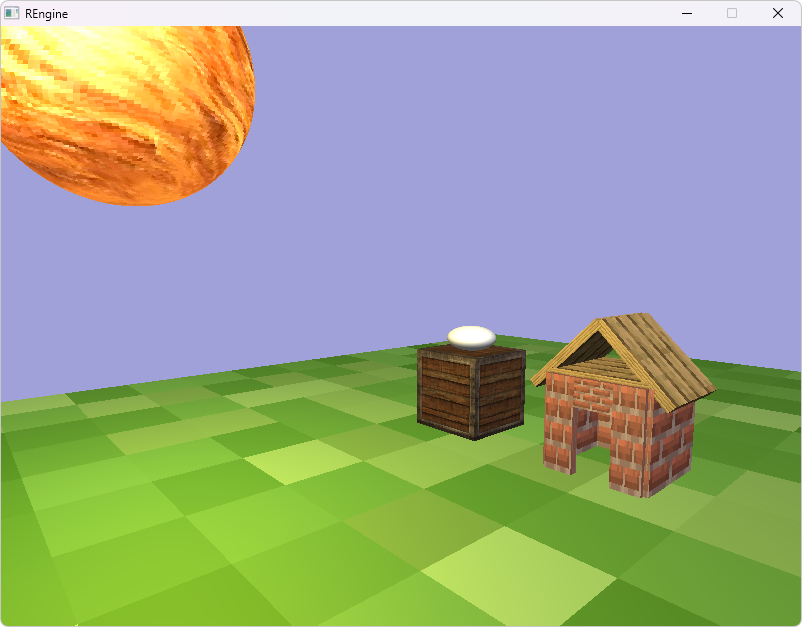
\includegraphics[width=1\linewidth]{scene.png}}
\caption{Загруженная сцена}
\label{scene:image}
\end{figure}

На рисунке \ref{culling:image} представлена сцена, тестирующая функционал отсечения невидимых поверхностей.

\begin{figure}[ht]
\center{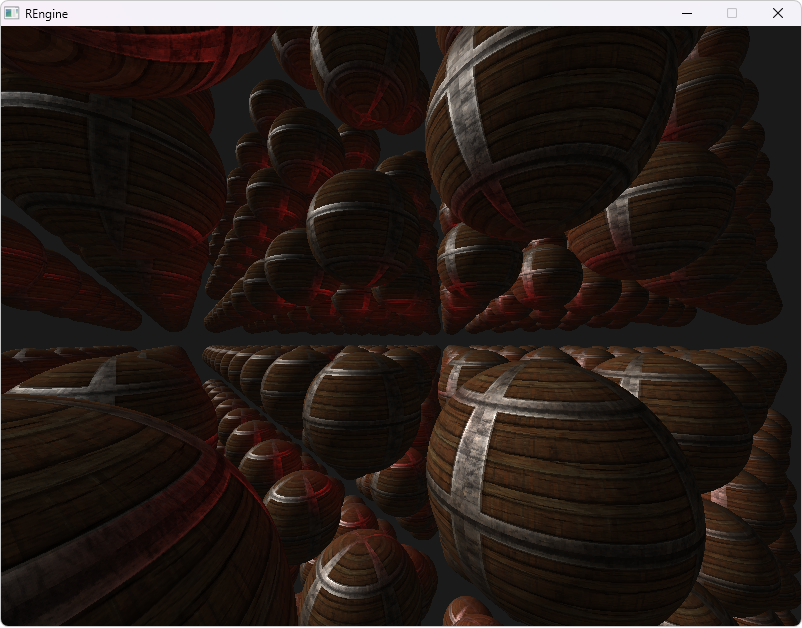
\includegraphics[width=1\linewidth]{culling.png}}
\caption{Сцена, тестирующая функционал отсечения невидимых поверхностей}
\label{culling:image}
\end{figure}

   \section*{ЗАКЛЮЧЕНИЕ}
\addcontentsline{toc}{section}{ЗАКЛЮЧЕНИЕ}

В ходе выполнения выпускной квалификационной работы была разработана кроссплатформенная система визуализации трёхмерной графики, обеспечивающая эффективный рендеринг сложных сцен в реальном времени. Разработанное программное решение демонстрирует высокую производительность и расширяемость, что позволяет применять его в различных областях, включая разработку интерактивных приложений, научную визуализацию и образовательные проекты.

Основные результаты работы:

\begin{enumerate}
    \item Проведён всесторонний анализ современных технологий и подходов в области компьютерной графики:
    \begin{itemize}
        \item исследованы современные графические API (OpenGL, Vulkan, DirectX);
        \item проанализированы существующие игровые движки и фреймворки;
        \item выбран оптимальный стек технологий: C++17, OpenGL 3.3, SDL2, GLM, GLSL.
    \end{itemize}
    
    \item Разработана архитектура кроссплатформенного графического движка:
    \begin{itemize}
        \item определены ключевые модули системы: рендеринг, управление ресурсами, обработка ввода;
        \item разработана система управления жизненным циклом приложения;
        \item спроектированы интерфейсы для расширения функциональности.
    \end{itemize}
    
    \item Реализованы основные компоненты графического конвейера:
    \begin{itemize}
        \item разработана система управления шейдерами с поддержкой загрузки пользовательского кода;
        \item реализована подсистема загрузки и управления текстурами;
        \item создана система работы с геометрическими примитивами и буферами вершин.
    \end{itemize}
    
    \item Разработана система работы с камерой и освещением сцены:
    \begin{itemize}
        \item реализован динамический объект камеры, имеющий возможность изменения позиции и поля обзора;
        \item добавлена поддержка источников света (направленные и точечные), рассчитываемых по модели Блинна-Фонга.
    \end{itemize}
    
    \item Создана система загрузки и управления сценами:
    \begin{itemize}
        \item реализован загрузчик графических файлов формата BMP;
        \item проведена оптимизация загрузки ресурсов с помощью кеширования;
        \item добавлена поддержка различных типов объектов (модели, источники света, камера).
    \end{itemize}
    
    \item Реализована система обработки пользовательского ввода:
    \begin{itemize}
        \item добавлена поддержка клавиатуры и мыши;
        \item реализована система настройки управления;
        \item обеспечена плавность управления камерой.
    \end{itemize}
    
    \item Проведены тестирование и оптимизация работы движка:
    \begin{itemize}
        \item реализованы модульные тесты для всех компонентов;
        \item проведено профилирование производительности;
        \item выполнена оптимизация рендеринга (отсечение объектов за пределами кадра).
    \end{itemize}
\end{enumerate}

Все требования, объявленные в техническом задании, были полностью реализованы, все задачи, поставленные в начале разработки проекта, были также решены. Разработанный информационная система демонстрирует стабильную работу на различных аппаратных конфигурациях и операционных системах. Достигнута частота кадров, достаточная для интерактивной работы со сложными трёхмерными сценами.

Готовый рабочий проект представлен в виде программной библиотеки на C++. Исходный код находится в публичном доступе, поскольку опубликован в сети Интернет.

}\fi
\addcontentsline{toc}{section}{СПИСОК ИСПОЛЬЗОВАННЫХ ИСТОЧНИКОВ}

\begin{thebibliography}{9}
    \bibitem{opengl-es} Будирижанто, П. OpenGL ES 3.0. Руководство разработчика / П. Будирижанто, Г. Дэн. – Москва~: ДМК Пресс, 2015. – 448 с. – ISBN 978-5-97060-256-0. – Текст~: непосредственный.
    \bibitem{cpp} Доусон, М. Изучаем C++ через программирование игр / М. Доусон. – Санкт-Петербург~: Питер, 2022. – 352 с. – ISBN 978-5-4461-1791-8. – Текст~: непосредственный.
    \bibitem{lafore} Лафоре, Р. Объектно-ориентированное программирование в С++. Классика Computer Science / Р. Лафоре. – Санкт-Петербург~: Питер, 2022. – 928 с. – ISBN 978-5-4461-0927-2. – Текст~: непосредственный.
    \bibitem{shildt} Шилдт Герберт. C++. Базовый курс / Г. Шилдт. – Москва~: Диалектика-Вильямс, 2018. – 624 с. – ISBN 978-5-907114-15-9. – Текст~: непосредственный.
    \bibitem{deitel} Дейтел П. C++20 для программистов / П. Дейтел, Х. Дейтел. – Санкт-Петербург~: Питер, 2024. – 1056 с. – ISBN 978-5-4461-2359-9. – Текст~: непосредственный.
    \bibitem{macconnell} Макконнелл, Д. Анализ алгоритмов. Активный обучающий подход. 3-е дополненное издание / Д. Макконнелл. – Москва~: Техносфера, 2023. – 416 с. – ISBN 978-5-94836-216-8. – Текст~: непосредственный.
    \bibitem{kovalyov} Ковалев, М. М. Дискретная оптимизация: Целочисленное программирование / М. М. Ковалев. – Москва~: Ленанд, 2023. – 192 с. – ISBN 978-5-9710-7853-1. – Текст~: непосредственный.
    \bibitem{mitchell} Митчелл, Ш. Разработка игр на SDL / Ш. Митчелл. – Москва~: Пакет, 2013. – 256 с. – ISBN 978-1-84969-682-1. – Текст~: непосредственный.
    \bibitem{guidukov} Гайдуков, С. А. OpenGL. Профессиональное программирование трехмерной графики на C++ / С. А. Гайдуков. – Санкт-Петербург~: БХВ-Петербург, 2011. – ISBN 978-5-94157-363-4. – Текст~: электронный.
    \bibitem{discrete} Авдошин, С. М. Дискретная математика. Алгоритмы: теория и практика / С. М. Авдошин, А. А. Набебин. – Москва~: ДМК Пресс, 2019. – 282 с. – ISBN 978-5-97060-688-9. – Текст~: непосредственный.
    \bibitem{data} Манцнер, Т. Визуализация данных. Полный и исчерпывающий курс для начинающих / Т. Манцнер. – Москва~: Эксмо, 2023. – 464 с. – ISBN 978-5-04-106797-7. – Текст~: непосредственный.
    \bibitem{knuth} Кнут, Д. Э. Искусство программирования. Том 3. Сортировка и поиск / Д. Э. Кнут. – Москва~: Диалектика Вильямс, 2019. – 832 с. – ISBN 978-5-907144-41-5. – Текст~: непосредственный.
    \bibitem{grok} Бхаргава, А. Грокаем алгоритмы. 2-е изд. / А. Бхаргава. – Санкт-Петербург~: Питер, 2025. – 352 с. – ISBN 978-5-4461-4172-2. – Текст~: непосредственный.
    \bibitem{c} Ритчи, Д. М. Язык программирования C | Д. М. Ритчи, Б. У. Керниган – Москва~: Вильямс, 2019. – 288 с. – ISBN 978-5-907144-14-9. – Текст~: непосредственный.
    \bibitem{test} Кейнер, К. Тестирование программного обеспечения: контекстно ориентированный подход / К. Кейнер, Дж. Бах. – Санкт-Петербург~: Питер, 2025. – 352 с. – ISBN 978-5-4461-2165-6. – Текст~: непосредственный.
    \bibitem{csharp} Тюкачев, Н. А. C\#. Программирование 2D и 3D векторной графики. Учебное пособие для вузов, 5-е изд., стер. / Н. А. Тюкачев, В. Г. Хлебостроев. – Санкт-Петербург~: Лань, 2024. – 320 с. – ISBN 978-5-507-47565-0. – Текст~: непосредственный.
    \bibitem{game} Андрианова, Н. А. Как создаются игры. Основы разработки для начинающих игроделов / Н. А. Андрианова. – Москва~: Бомбора, 2023. – 336 с. – ISBN 978-5-04-120353-5. – Текст~: непосредственный.
    \bibitem{test2} Элфрид, Д. Автоматизированное тестирование программного обеспечения / Д. Элфрид, Р. Джефф, П. Джон. – Москва~: Лори, 2023. – 592 с. – ISBN 978-5-85582-409-4. – Текст~: непосредственный.
    \bibitem{req} Вигерс, К. И. Разработка требований к программному обеспечению. 3-е изд., дополненное / К. И. Вигерс, Дж. Битти. – Санкт-Петербург~: БХВ, 2024. – 736 с. – ISBN 978-5-9909805-3-2. – Текст~: непосредственный.
    \bibitem{wolf} Вольф, Д. OpenGL 4. Язык шейдеров. Книга рецептов / Д. Вольф. – Москва~: ДМК Пресс, 2017. – ISBN 978-5-97060-255-3. – Текст~: электронный.
\end{thebibliography}

\ifВКР{\appendix{Представление графического материала}

Графический материал, выполненный на отдельных листах,
изображен на рисунках А.1--А.\arabic{числоПлакатов}.
\setcounter{числоПлакатов}{0}

\renewcommand{\thefigure}{А.\arabic{figure}} % шаблон номера для плакатов

\begin{landscape}

\begin{плакат}
    \includegraphics[width=0.82\linewidth]{p1}
    \заголовок{Сведения о ВКРБ}
    \label{pl1:image}
\end{плакат}

\begin{плакат}
    \includegraphics[width=0.82\linewidth]{p2}
    \заголовок{Цель и задачи разработки}
    \label{pl2:image}
\end{плакат}

\begin{плакат}
    \includegraphics[width=0.82\linewidth]{p3}
    \заголовок{Диаграмма компонентов}
    \label{pl3:image}
\end{плакат}

\begin{плакат}
    \includegraphics[width=0.82\linewidth]{p4}
    \заголовок{Диаграмма классов}
    \label{pl4:image}
\end{плакат}

\begin{плакат}
    \includegraphics[width=0.82\linewidth]{p5.png}
    \заголовок{Изображение основной сцены}
    \label{pl5:image}
\end{плакат}

\begin{плакат}
    \includegraphics[width=0.82\linewidth]{p6.png}
    \заголовок{Тестирование оптимизации}
    \label{pl6:image}
\end{плакат}

\begin{плакат}
    \includegraphics[width=0.82\linewidth]{p7}
    \заголовок{Заключение}
    \label{pl7:image}
\end{плакат}

\end{landscape}
}\fi
\ifПрактика{}\else{\appendix{Фрагменты исходного кода программы}

Engine.cpp
\lstinputlisting[language=C++, frame=none]{../src/Engine.cpp}

Renderer.cpp
\lstinputlisting[language=C++, frame=none]{../src/Renderer.cpp}

\ifВКР{
\newpage
\addcontentsline{toc}{section}{На отдельных листах (CD-RW в прикрепленном конверте)}
\noindent
\begin{tabular}{p{5.8cm}C{4.8cm}C{4.8cm}}
   Автор ВКР & \lhrulefill{\fill} & \fillcenter\Автор \\
            \setarstrut{\footnotesize}
           & \footnotesize{(подпись, дата)} & \\
            \restorearstrut
   Руководитель ВКР & \lhrulefill{\fill} & \fillcenter\Руководитель \\
            \setarstrut{\footnotesize}
           & \footnotesize{(подпись, дата)} & \\
            \restorearstrut
   Нормоконтроль & \lhrulefill{\fill} & \fillcenter\Нормоконтроль \\
            \setarstrut{\footnotesize}
           & \footnotesize{(подпись, дата)} & \\
            \restorearstrut
\end{tabular}
\vskip 2cm
\begin{center}
\textbf{Место для диска}
\end{center}
}\fi
}\fi
\end{document}
